\documentclass[12pt]{article}
\usepackage{latex/ntgclass/a4}
\usepackage{epsfig}
%\usepackage{graphicx}
%\usepackage{floatfig}
%\usepackage{floatflt}
\usepackage{latex/subfigure/subfigure}
\usepackage{latex/multirow/multirow}
%\usepackage{rotate}
%\usepackage{rotating}
%\usepackage{doublespace}
\usepackage{latex/setspace/setspace}
\usepackage{latex/fancyvrb}
\usepackage{latex/caption}
\usepackage{latex/caption3}

%\include{latex/header}
% \documentstyle[a4,12pt,latex/nimr,subfigure,titlepage,epsf]{article}
% \documentstyle[a4,12pt,latex/nimr,subfigure,titlepage,doublespace]{article}

\newcommand{\Part}[1]{Part~\ref{Part:#1}}
\newcommand{\App}[1]{Appendix~\ref{App:#1}}
\newcommand{\Eqn}[1]{Equ$^n$.~\ref{Eqn:#1}}
\newcommand{\Sec}[1]{Section~\ref{Sec:#1}}
\newcommand{\Met}[1]{Methods Sect$^n$.~\ref{Met:#1}}
\newcommand{\Res}[1]{Results Sect$^n$.~\ref{Res:#1}}
\newcommand{\Tab}[1]{Table~\ref{Tab:#1}}
\newcommand{\Fig}[1]{Figure~\ref{Fig:#1}}
\newcommand{\Mbox}[1]{Box~\ref{Box:#1}}
\newcommand{\Tbox}[1]{Box~\ref{Box:#1}}
\newcommand{\SupMat}[1]{Supplementary Material~\ref{SupMat:#1}}
\newcommand{\SupFig}[1]{Supplementary Figure~\ref{SupFig:#1}}
\newcommand{\Sup}[1]{Supplementary Figure~\ref{Sup:#1}}

\newcommand{\Aa}[1]{{\footnotesize #1}}
\newcommand{\HB}{hydrogen-bond}
\newcommand{\AC}{$\alpha$-carbon}
\newcommand{\BC}{$\beta$-carbon }
\newcommand{\CA}{$\alpha$-carbon}
\newcommand{\ca}{$\alpha$-carbon}
\newcommand{\CB}{$\beta$-carbon}
\newcommand{\Ca}{C$_\alpha$}
\newcommand{\Cb}{C$_\beta$}
\newcommand{\AH}{$\alpha$-helix}
\newcommand{\AHs}{$\alpha$-helices}
\newcommand{\BS}{$\beta$-sheet}
\newcommand{\Bs}{$\beta$-strand}
\newcommand{\A}{$\alpha$}
\newcommand{\B}{$\beta$}
\newcommand{\3}{$3_{10}$}
\newcommand{\BAB}{$\beta\alpha\beta$}
\newcommand{\BA}{$\beta$/$\alpha$}
\newcommand{\degree}{$^\circ$}
\newcommand{\degre}{$^\circ$}
\newcommand{\UP}[1]{\;^{#1}\!}
\newcommand{\UUP}[1]{\;^{^{#1}\!}\!}
\newcommand{\BL}{{\tt BLAST}}
\newcommand{\MST}{{\tt MST}}
\newcommand{\PBL}{$\Psi$-{\tt BLAST}}
\newcommand{\BLAST}{{\tt BLAST}}
\newcommand{\REP}{{\tt REPRO}}
\newcommand{\MUL}{{\tt MULTAL}}
\newcommand{\SEL}{{\tt MULSEL}}
\newcommand{\SAP}{{\tt SAP}}
\newcommand{\TMA}{{\tt TMalign}}
\newcommand{\DALI}{{\tt DALI}}
\newcommand{\SSAP}{{\tt SSAP}}
\newcommand{\POPS}{{\tt POPS}}
\newcommand{\JEGT}{{\small JGET}$_{95}$}
\newcommand{\DSSP}{{\tt DSSP}}
\newcommand{\STICK}{{\tt STICK}}
\newcommand{\TUNE}{{\tt TUNE-3D}}
\newcommand{\SPREK}{{\tt SPREK}}
\newcommand{\QUEST}{{\tt QUEST}}
\newcommand{\PHOBIC}{{\tt PHOBIC}}
\newcommand{\SPRATT}{{\tt SPRATT}}
\newcommand{\PRATT}{{\tt PRATT}}
\newcommand{\DRAGON}{{\tt DRAGON}}
\newcommand{\RAMBLE}{{\tt RAMBLE}}
\newcommand{\GADGET}{{\tt GADGET}}
\newcommand{\PSIPRED}{{\tt PSIPRED}}
\newcommand{\RASMOL}{{\tt RASMOL}}
\newcommand{\CAMPAS}{{\small CAMPASS}}
\newcommand{\HOM}{{\small HOMSTRAD}}
\newcommand{\PLATO}{{\small PLATO}}
\newcommand{\RE}{regular-expression}
\newcommand{\REM}{regular-expression matching}
\newcommand{\SAM}{{\tt SAM}}
\newcommand{\SWP}{SWISS-PROT}
\newcommand{\eg}{{\em e.~g.}}
\newcommand{\fiveP}{$5'$}
\newcommand{\threP}{$3'$}

\newcommand{\dgr}{\mbox{$^{\circ}$}}                    % degrees
\newcommand{\al}{\mbox{$\alpha$}}                       % alpha
\newcommand{\be}{\mbox{$\beta$}}                        % beta
\newcommand{\tten}{\mbox{$3_{10}$}}                     % 3-ten
\newcommand{\bal}{\mbox{\protect\boldmath $\alpha$}}    % bold alpha
\newcommand{\bbe}{\mbox{\protect\boldmath $\beta$}}     % bold beta
\newcommand{\btten}{\mbox{\protect\boldmath $3_{10}$}}  % bold 3-ten
\newcommand{\RMSD}{\mbox{\rm RMSD}}                     % rmsd
\newcommand{\RMS}{\mbox{\rm RMS}}                       % rms
\newcommand{\RMSS}{\mbox{\rm RMS$_{\rm S}$}}            % rms superposition
\newcommand{\RMSDM}{\mbox{\rm RMS$_{\rm DM}$}}          % rms difference matrix
\newcommand{\DK}{\mbox{\rm D$_{k}$}}                    % sippl82 Dk
\newcommand{\RMSG}{\mbox{\rm RMS$_{\rm S\mbox{$^{\rm *}$}}$}}  % rms multiple

\newcommand{\SSS}{super-secondary structure}
\newcommand{\FT}{Fourier transform}                                                                 
% \newcommand{\epsfxsize}{Figure}
% \newcommand{\epsfbox}[1]{{will be file {#1}}}
% \newcommand{\includegraphics}[1]{{Figure will be file {#1}}}

\newcommand{\mA}{{\bf A}}
\newcommand{\mB}{{\bf B}}
\newcommand{\mC}{{\bf C}}
\newcommand{\mD}{{\bf D}}
\newcommand{\mE}{{\bf E}}
\newcommand{\mM}{{\bf M}}
\newcommand{\mP}{{\bf P}}
\newcommand{\mQ}{{\bf Q}}
\newcommand{\mR}{{\bf R}}
\newcommand{\mS}{{\bf S}}
\newcommand{\mT}{{\bf T}}
\newcommand{\mU}{{\bf U}}
\newcommand{\mV}{{\bf V}}
\newcommand{\mW}{{\bf W}}

\newcommand{\va}{{\bf a}}
\newcommand{\vb}{{\bf b}}
\newcommand{\vc}{{\bf c}}
\newcommand{\vd}{{\bf d}}
\newcommand{\ve}{{\bf e}}
\newcommand{\vf}{{\bf f}}
\newcommand{\vg}{{\bf g}}
\newcommand{\vh}{{\bf h}}
\newcommand{\vm}{{\bf m}}
\newcommand{\vo}{{\bf o}}
\newcommand{\vp}{{\bf p}}
\newcommand{\vq}{{\bf q}}
\newcommand{\vr}{{\bf r}}
\newcommand{\vs}{{\bf s}}
\newcommand{\vt}{{\bf t}}
\newcommand{\vu}{{\bf u}}
\newcommand{\vv}{{\bf v}}
\newcommand{\vw}{{\bf w}}
\newcommand{\vx}{{\bf x}}
\newcommand{\vy}{{\bf y}}
\newcommand{\vz}{{\bf z}}

\usepackage{lmodern}
\renewcommand\ttfamily{\usefont{T1}{lmtt}{m}{n}}

\setstretch{1.5}

\begin{document}

\title{\bf A comparative analysis of the foamy and ortho virus capsid structures
           reveals an ancient domain duplication.
}

\author{\\William~R.~Taylor$^{\dagger*}$,
Jonathan~P.~Stoye$^{\ddagger}$\\
and
Ian~A.~Taylor$^{\S}$\\ \\ \\ \\
$^\dagger$Computational Cell and Molecular Biology,\\
$^\ddagger$Virology, and
$^\S$Molecular Structure Laboratories,\\
Francis Crick Institute,\\
1 Midland Rd., London NW1 1AT, UK.\\ \\ \\
$^*$ corresponding author: william.taylor@crick.ac.uk\\ \\ \\ \\
{\bf Keywords:} Virus capsid structure; foamy virus;\\ protein structure comparison.\\ \\ \\
}
\begin{singlespace}
\maketitle
\end{singlespace}
\clearpage
%The {\em Spumaretrovirinae} (foamy viruses) and the {\em Orthoretrovirinae} (e.g. HIV) share
many similarities both in genome structure and the sequences of the core viral encoded proteins,
such as the aspartyl protease and reverse-transcriptase.  Similarity in the Gag region of the 
genome is less obvious at the sequence level but has been illuminated by the recent solution of
the foamy virus capsid (CA) structure.   This revealed a clear structural similarity to the 
orthoretrovirus capsids but with marked differences that left uncertainty in the relationship
between the two domains that comprise the structure.   Using multiple structure comparison
methods combined with statistical tests, we have shown that the relationship of the two domains
conforms to a simple linear correspondance rather than a domain transposition.   These
similarities suggest that the origin of both viral capsids was a common ancestor with a double
domain structure.  In addition, we show that there is also a significant structural similarity 
between the amino and carboxy domains in both the foamy and ortho viruses which suggests that
there may have been an even more ancient gene-duplication that preceded the double domain structure.

\clearpage
%\section{Introduction}

Taxonomically, the {\em Orthoretrovirinae} (orthoretroviruses) and {\em Spumaretrovirinae}\footnote{
This class is also commonly referred to as the Foamy viruses (after the morphological effect they have on infected cells)
and will be referred by this name frequently below, with the term orthoretroviruses also contracted to "Ortho viruses".
} 
(spumaviruses) make up the two subfamilies of {\em Retroviridae}. They share many similarities, including overall genome
structures with gag, pol and env genes encoding proteins for replication and life cycles involving reverse transcription
and integration into the chromosomes of infected cells. However, there are also a number of differences distinguishing these
viral subfamilies, including finer details of genome organisation, the absence of a Gag-Pol fusion protein in spumaviruses
and the timing of reverse transcription.

Gag is the major structural protein of both Ortho and Foamy viruses and also displays both important differences and similarities.
Ortho and Foamy viral Gag are required for particle assembly, budding from the cell, reverse transcription and delivery of the
viral nucleic acid into the newly infected cell. However, there are a number of striking differences including how the Gag
precursor is targeted to the cell membrane, the absence of a Major Homology Region and Cys-His box in Foamy viruses and very 
different patterns of processing during viral maturation. In all Ortho viruses, Gag is proteolytically cleaved to form distinct, 
well-studied proteins, matrix (MA), capsid (CA) and nucleocapsid (NC), found in mature virions but in spumaviruses Gag processing 
does not occur. 

The recent solution of the Foamy Gag protein structure has shed new light on this relationship by revealing that
the capsid structures of both viral classes share a common protein fold, with the implication that their gag proteins may
be evolutionarily related \cite{BallNJet16}.   An intriguing aspect of this relationship was an ambiguity in the degree of
relatedness between the two domains of the gag proteins, with the Spumaretroviral Gag domains appearing almost equally
similar to both the amino- and carboxy-terminal domains of the orthoretroviruses.   In this paper, we investigate the
nature of this relationship in greater detail and discuss its evolutionary implications. 

\section{Introduction}

Taxonomically, the {\em Orthoretrovirinae} (orthoretroviruses) and {\em Spumaretrovirinae}\footnote{
This class is also commonly referred to as the Foamy viruses (after the morphological effect they have on infected cells)
and will be referred by this name frequently below, with the term orthoretroviruses also contracted to "Ortho viruses".
} 
(spumaviruses) make up the two subfamilies of {\em Retroviridae}. They share many similarities, including overall genome
structures with gag, pol and env genes encoding proteins for replication and life cycles involving reverse transcription
and integration into the chromosomes of infected cells. However, there are also a number of differences distinguishing these
viral subfamilies, including finer details of genome organisation, the absence of a Gag-Pol fusion protein in spumaviruses
and the timing of reverse transcription.

Gag is the major structural protein of both Ortho and Foamy viruses and also displays both important differences and similarities.
Ortho and Foamy viral Gag are required for particle assembly, budding from the cell, reverse transcription and delivery of the
viral nucleic acid into the newly infected cell. However, there are a number of striking differences including how the Gag
precursor is targeted to the cell membrane, the absence of a Major Homology Region and Cys-His box in Foamy viruses and very 
different patterns of processing during viral maturation. In all Ortho viruses, Gag is proteolytically cleaved to form distinct, 
well-studied proteins, matrix (MA), capsid (CA) and nucleocapsid (NC), found in mature virions but in spumaviruses Gag processing 
does not occur. 

The recent solution of the Foamy Gag protein structure has shed new light on this relationship by revealing that
the capsid structures of both viral classes share a common protein fold, with the implication that their gag proteins may
be evolutionarily related \cite{BallNJet16}.   An intriguing aspect of this relationship was an ambiguity in the degree of
relatedness between the two domains of the gag proteins, with the Spumaretroviral Gag domains appearing almost equally
similar to both the amino- and carboxy-terminal domains of the orthoretroviruses.   In this paper, we investigate the
nature of this relationship in greater detail and discuss its evolutionary implications. 
\clearpage
%\include{results}
\section{Results}

\subsection{Full-length comparison}

To investigate the structural relationship between the capsid structure of the ortho viruses (HIV, MLV, etc.),
and the new structure of the foamy virus capsid \cite{BallNJet16} (PDB codes: 5m1g, 5m1h), the foamy virus structure was
compared to one of the few full double domain ortho virus structures, the HIV capsid with PDB code: {\tt 3nte},
using the flexible superposition program \SAP\ \cite{TaylorWR99a}.   Even though this program has a tolerant approach
to relative domain shifts, the comparison produced a high RMSD value of 14\AA\ over the 100 best superposed
positions.   The amino (N) terminal domain positions roughly corresponded but shifts in the relative
orientation of the carboxy (C) terminal domain resulted in large deviations between equivalent helices.  
The superposed structures are shown in \Fig{fullSAP} and the domain divergence can be seen clearly as a
jump in the cumulative RMSD plot (\Fig{fullRMS}).

\begin{figure}
\centering
\subfigure[]{
\label{Fig:fullSAP}
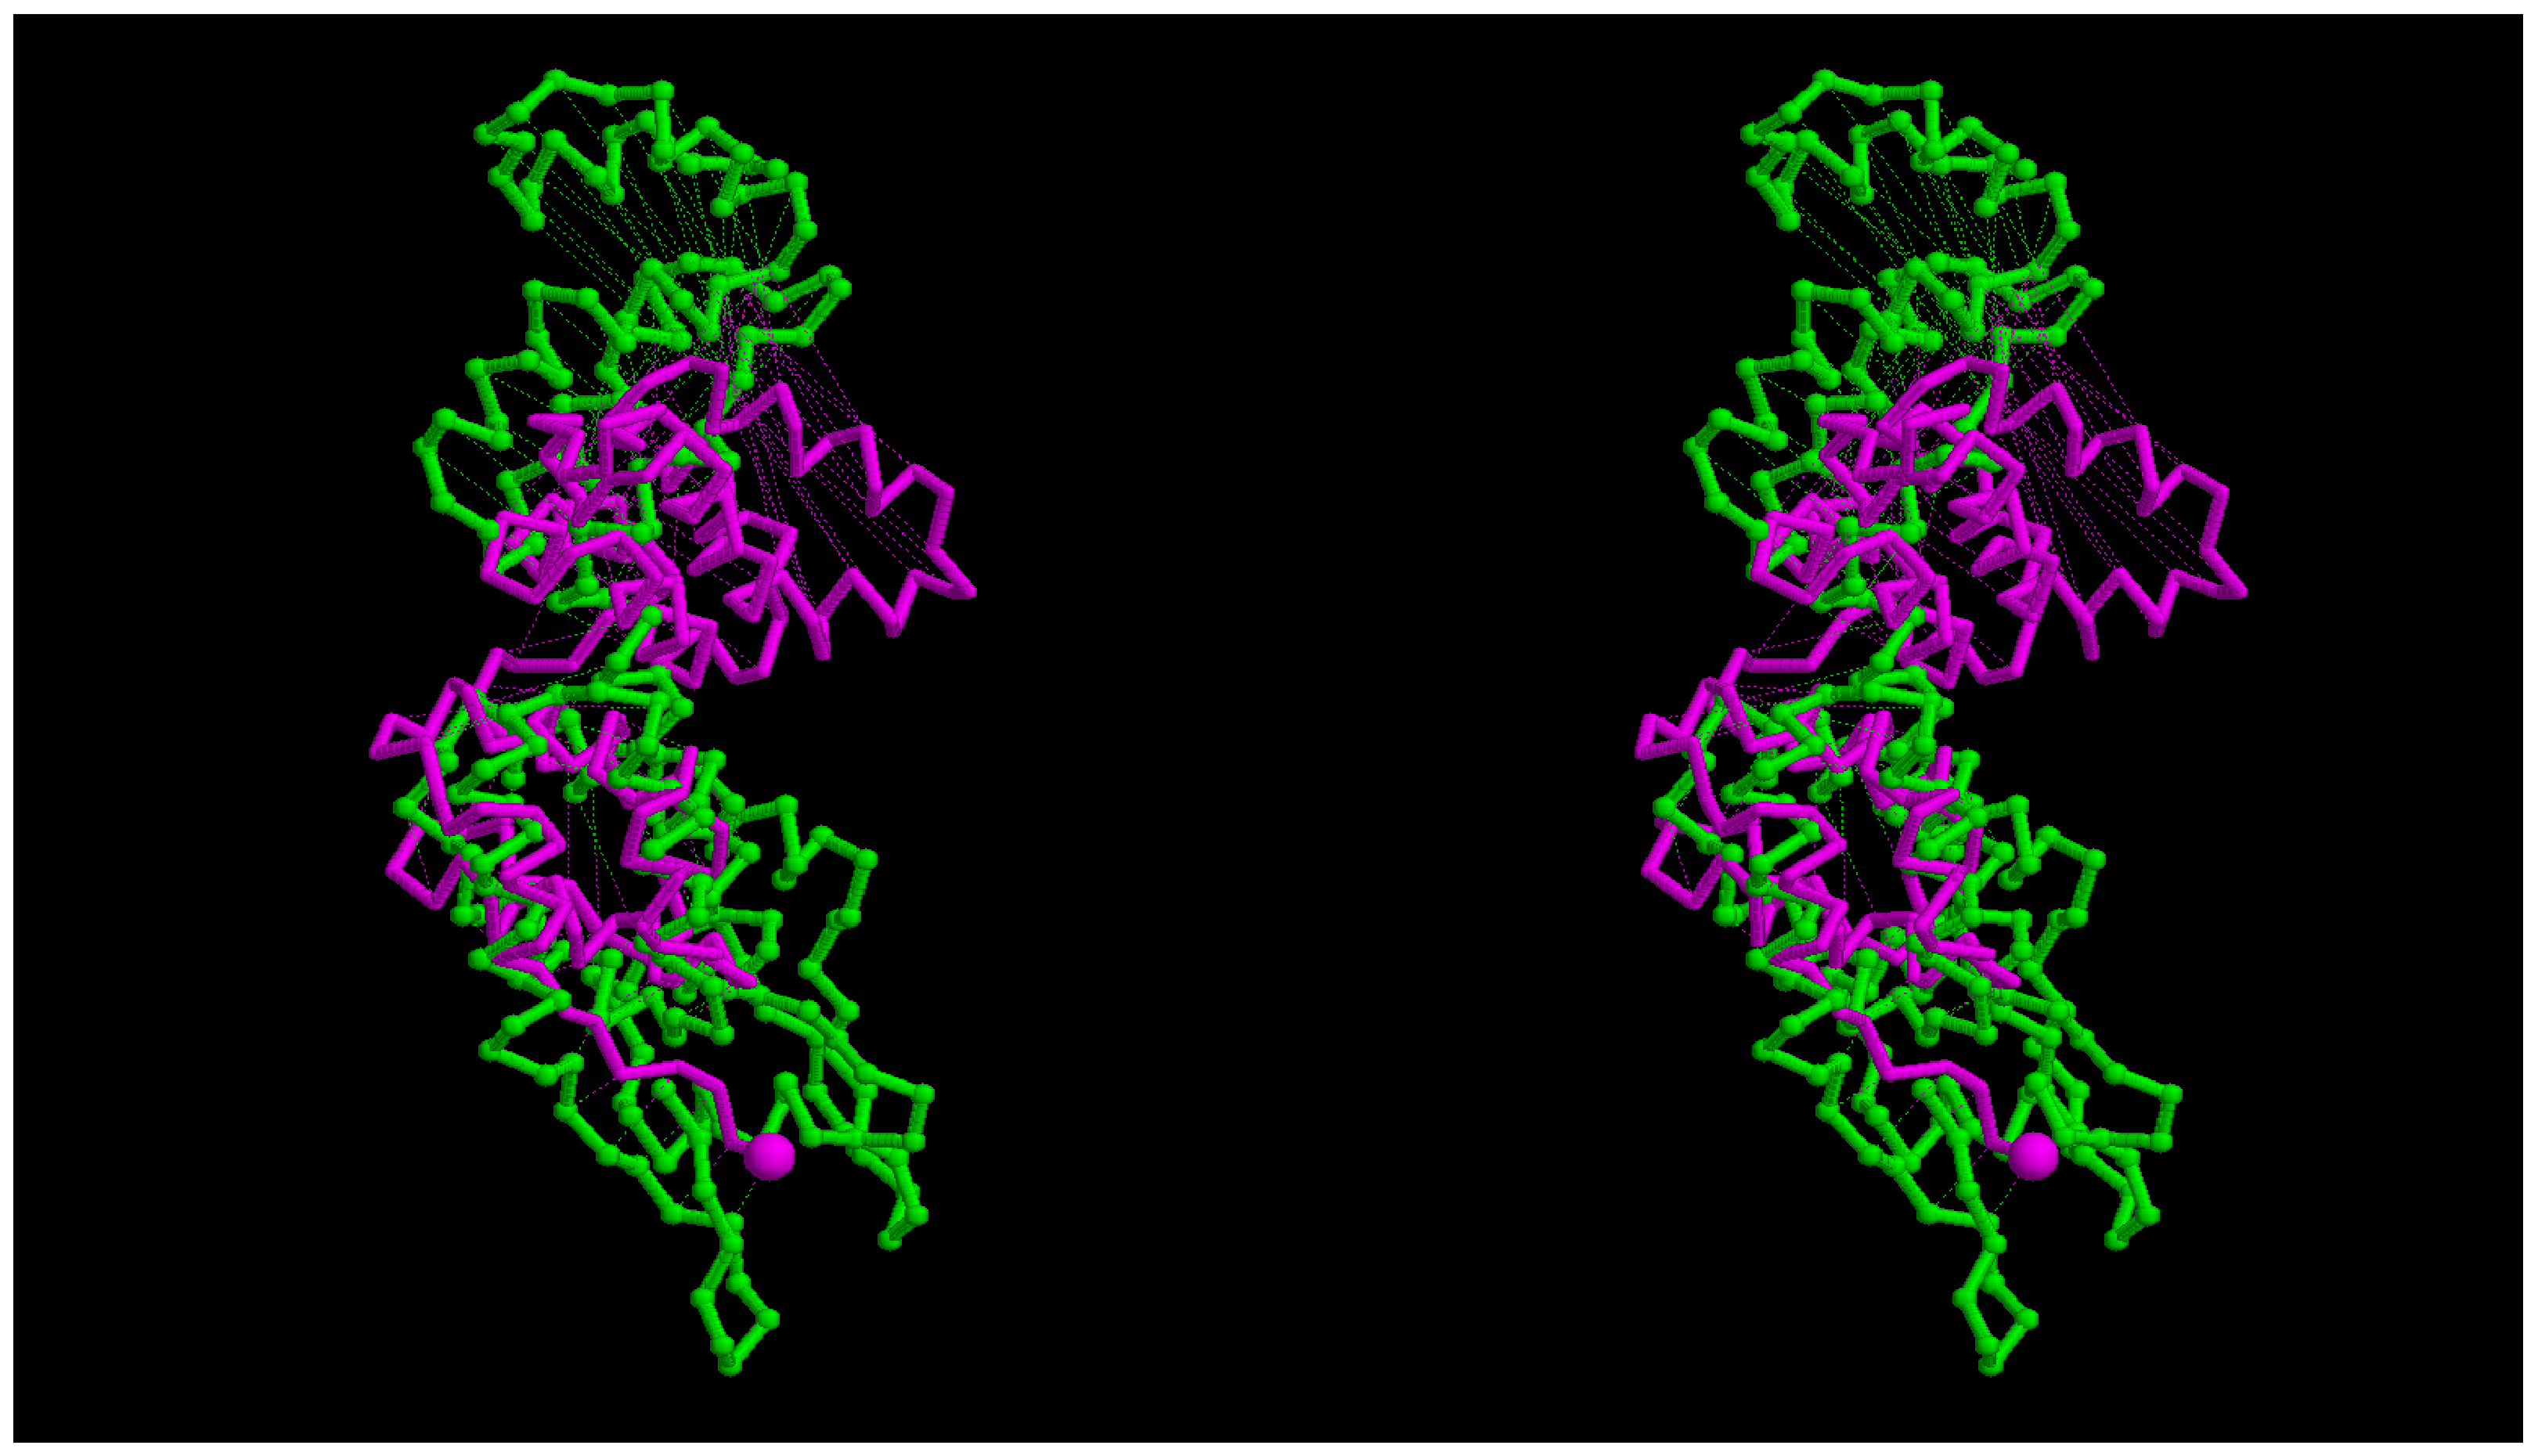
\includegraphics[width=300pt]{full3nte-super.eps}
}
\subfigure[]{
\label{Fig:fullRMS}
\rotatebox{270}{
\includegraphics[width=220pt]{plotrms.eps}
}}
\begin{footnotesize}
\caption{
\label{Fig:full}
{\bf Full ortho/foamy virus capsid superposition}.
The superposed structures are shown in part ($a$) as a stereo pair, coloured as green = ortho virus (HIV, PDB code: {\tt 3nte-A})
and magenta = foamy virus capsid.   (The amino terminus is marked by a small sphere).
Part ($b$) shows the cumulative RMSD plot for this superposition which plots the RMSD value (Y-axis) for increasingly larger sets
of residues as ranked by their \SAP\ similarity score (X-axis).   The sharp rise in this trace marks the transition into 
subsets that include positions from the displaced domain.
}
\end{footnotesize}
\end{figure}

\subsection{DALI searches}

Although this initial superposition (\Fig{full}) did not appear encouraging, the foamy virus structure
was scanned across the Protein DataBank (PDB), using the \DALI\ program \cite{HolmLet93a} to search for any similarities.

\subsubsection{Full chain scan}

A scan of the full-length foamy structure using the DALI server\footnote{
{\tt http://ekhidna.biocenter.helsinki.fi/dali\_server},
see Methods section for details.
}
over the 90\% non-redundant protein structure databank
identified a wide selection of retroviral capsid structures.  In the ranked list of structure hits,
capsids were identified from position 2 to position 550.
The top hits are shown in \Fig{dali} (See Supplementary material for a summary of
the full 550 with Z-scores over 2).    Many capsids are found in the top 20 hits and although the top
scoring hit is not obviously a capsid protein, it is thought to have originated from the Ty3/Gypsy
retrotransposon family gag gene \cite{ZhangWet15}.   However, almost all of these are partial
hits, covering little more than half the query structure.   The structural alignment of the top two hits
is shown in \Fig{top2} coloured to emphasise the matched regions.

\begin{figure}
\centering
\begin{singlespace}
\begin{tiny}
\begin{Verbatim}[frame=single]
   No:  Chain   Z    rmsd lali nres  %id PDB  Description
    1:  4x3x-A  5.0  3.1   66    82   11 PDB  MOLECULE: ACTIVITY-REGULATED CYTOSKELETON-ASSOC
    2|  3g29-A  3.7  2.7   60    77    8 PDB  MOLECULE: GAG POLYPROTEIN;                                           
    3|  3g0v-A  3.7  2.9   62    76    8 PDB  MOLECULE: GAG POLYPROTEIN;                                           
    4:  2v50-D  3.6  2.2   41   998    7 PDB  MOLECULE: MULTIDRUG RESISTANCE PROTEIN MEXB;                         
    5:  3j39-i  3.6  2.5   40   113    3 PDB  MOLECULE: 60S RIBOSOMAL PROTEIN L10A-2;                              
    6|  4ph2-A  3.6  3.2   69   127    7 PDB  MOLECULE: BLV CAPSID - N-TERMINAL DOMAIN;                            
    7:  1iqp-E  3.6  3.8   69   326    7 PDB  MOLECULE: RFCS;                                                      
    8:  4gco-A  3.6  3.7   55   120   11 PDB  MOLECULE: PROTEIN STI-1;                                             
    9|  3g29-B  3.6  2.8   62    77    8 PDB  MOLECULE: GAG POLYPROTEIN;                                           
   10|  3g1i-B  3.6  2.9   62    75    8 PDB  MOLECULE: GAG POLYPROTEIN;                                           
   11|  3g21-A  3.6  2.8   60    77    8 PDB  MOLECULE: GAG POLYPROTEIN;                                           
   12:  2a0u-A  3.5  3.1   68   374    4 PDB  MOLECULE: INITIATION FACTOR 2B;                                      
   13:  1j7q-A  3.5  2.9   60    86    5 PDB  MOLECULE: CALCIUM VECTOR PROTEIN;                                    
   14:  2a0u-B  3.5  8.1   80   367    4 PDB  MOLECULE: INITIATION FACTOR 2B;                                      
   15:  1iqp-A  3.5  3.7   70   326    7 PDB  MOLECULE: RFCS;                                                      
   16|  4ph0-C  3.5  4.6  101   199    8 PDB  MOLECULE: BLV CAPSID;                                                
   17|  4ph0-D  3.5  4.2  101   198    8 PDB  MOLECULE: BLV CAPSID;                                                
   18|  4ph2-B  3.5  3.3   69   127    7 PDB  MOLECULE: BLV CAPSID - N-TERMINAL DOMAIN;                            
   19:  1sxj-B  3.4  3.5   65   316    3 PDB  MOLECULE: ACTIVATOR 1 95 KDA SUBUNIT;                                
   20:  2afd-A  3.4  2.7   59    88   14 PDB  MOLECULE: PROTEIN ASL1650;                                           
\end{Verbatim}
\end{tiny}
\end{singlespace}
\begin{footnotesize}
\caption{
\label{Fig:dali}
{\bf Top structural similarities}
found by the \DALI\ program in the 90\% non-redundant PDB (PDB-90) using the full length foamy
virus capsid as a query (145 residues).
The columns are: the ranked number of the hit ({\tt No.}), marked by a '{\tt |}' for a capsid protein, otherwise '{\tt :}';
the PDB entry identifier ({\tt Chain}, with the chain designation after the dash); the \DALI\ Z-score ({\tt Z})
(significance estimate); the root-mean-square-deviation ({\tt rmsd}) over aligned \CA\ positions; the number
of aligned positions ({\tt lali}); the number of residues in the matched structure ({\tt nres}); the percentage
sequence identity of the match ({\tt \%id}) followed by a description of the molecule.
It can be seen from the number of matched positions ({\tt lali}) that most matches are partial, 
covering typically less than half the query structure.
}
\end{footnotesize}
\end{figure}

% query = new.cas
% 
% Nterm = PIGTVIPIQHIRSVTGEPPRNPREIPIWLGRNAPAIDGVFPVTTPDLRCRIINAILGGNIGLSLTPGDCLTWDSAVATLFIRTHGT
% Cterm = FPMHQLGNVIKGIVDQEGVATAYTLGMMLSGQNYQLVSGIIRGYLPGQAVVTALQQRLDQEIDNQTRAETFIQHLNAVYEILGLNARGQSIRLE
% 
% Matches to PDB90
% 
%   No:  Chain   Z    rmsd lali nres  %id PDB  Description
%    1:  4x3x-A  5.0  3.1   66    82   11 PDB  MOLECULE: ACTIVITY-REGULATED CYTOSKELETON-ASSOCIATED PROTEI          
%    2|  3g29-A  3.7  2.7   60    77    8 PDB  MOLECULE: GAG POLYPROTEIN;                                           
%    3|  3g0v-A  3.7  2.9   62    76    8 PDB  MOLECULE: GAG POLYPROTEIN;                                           
%    4:  2v50-D  3.6  2.2   41   998    7 PDB  MOLECULE: MULTIDRUG RESISTANCE PROTEIN MEXB;                         
%    5:  3j39-i  3.6  2.5   40   113    3 PDB  MOLECULE: 60S RIBOSOMAL PROTEIN L10A-2;                              
%    6|  4ph2-A  3.6  3.2   69   127    7 PDB  MOLECULE: BLV CAPSID - N-TERMINAL DOMAIN;                            
%    7:  1iqp-E  3.6  3.8   69   326    7 PDB  MOLECULE: RFCS;                                                      
%    8:  4gco-A  3.6  3.7   55   120   11 PDB  MOLECULE: PROTEIN STI-1;                                             
%    9|  3g29-B  3.6  2.8   62    77    8 PDB  MOLECULE: GAG POLYPROTEIN;                                           
%   10|  3g1i-B  3.6  2.9   62    75    8 PDB  MOLECULE: GAG POLYPROTEIN;                                           
%   11|  3g21-A  3.6  2.8   60    77    8 PDB  MOLECULE: GAG POLYPROTEIN;                                           
%   12:  2a0u-A  3.5  3.1   68   374    4 PDB  MOLECULE: INITIATION FACTOR 2B;                                      
%   13:  1j7q-A  3.5  2.9   60    86    5 PDB  MOLECULE: CALCIUM VECTOR PROTEIN;                                    
%   14:  2a0u-B  3.5  8.1   80   367    4 PDB  MOLECULE: INITIATION FACTOR 2B;                                      
%   15:  1iqp-A  3.5  3.7   70   326    7 PDB  MOLECULE: RFCS;                                                      
%   16|  4ph0-C  3.5  4.6  101   199    8 PDB  MOLECULE: BLV CAPSID;                                                
%   17|  4ph0-D  3.5  4.2  101   198    8 PDB  MOLECULE: BLV CAPSID;                                                
%   18|  4ph2-B  3.5  3.3   69   127    7 PDB  MOLECULE: BLV CAPSID - N-TERMINAL DOMAIN;                            
%   19:  1sxj-B  3.4  3.5   65   316    3 PDB  MOLECULE: ACTIVATOR 1 95 KDA SUBUNIT;                                
%   20:  2afd-A  3.4  2.7   59    88   14 PDB  MOLECULE: PROTEIN ASL1650;                                           
%   21:  2yhe-A  3.4  2.8   40   639    8 PDB  MOLECULE: SEC-ALKYL SULFATASE;                                       
%   22:  4u8y-B  3.4  4.4   64  1033    3 PDB  MOLECULE: MULTIDRUG EFFLUX PUMP SUBUNIT ACRB;                        
%   23:  2yhe-C  3.4  7.1   70   634    6 PDB  MOLECULE: SEC-ALKYL SULFATASE;                                       
%   24:  2yhe-E  3.4  6.6   72   634    7 PDB  MOLECULE: SEC-ALKYL SULFATASE;                                       
%   25|  4coc-B  3.4  3.1   64    79    9 PDB  MOLECULE: CAPSID PROTEIN P24;                                        
%   26:  4av7-D  3.4  8.1   70   634    7 PDB  MOLECULE: SEC-ALKYLSULFATASE;                                        
%   27:  4mbq-F  3.4  3.2   42    50    5 PDB  MOLECULE: MOTILITY PROTEIN FIMV;                                     
%   28|  3g1g-B  3.4  2.9   61    75    8 PDB  MOLECULE: GAG POLYPROTEIN;                                           
%   29:  2w8a-A  3.3  2.0   43   531    7 PDB  MOLECULE: GLYCINE BETAINE TRANSPORTER BETP;                          
%   30|  3ce7-A  3.3  2.7   59    90    5 PDB  MOLECULE: SPECIFIC MITOCHODRIAL ACYL CARRIER PROTEIN;                
%   31:  1eia-A  3.3  2.8   62   207   11 PDB  MOLECULE: EIAV CAPSID PROTEIN P26;                                   
%   32:  1k6y-B  3.3  2.4   40   194    3 PDB  MOLECULE: INTEGRASE;                                                 
%   33:  2lo0-A  3.3  2.5   33    45    6 PDB  MOLECULE: UNCHARACTERIZED PROTEIN;                                   
%   34:  3w9j-B  3.3  4.3   64  1030    5 PDB  MOLECULE: MULTIDRUG RESISTANCE PROTEIN MEXB;                         
%   35:  4dx6-B  3.3  4.6   67  1033    4 PDB  MOLECULE: ACRIFLAVINE RESISTANCE PROTEIN B;                          
%   36:  1iqp-D  3.3  3.9   70   326    7 PDB  MOLECULE: RFCS;                                                      
%   37:  2afe-A  3.3  2.8   59    88   12 PDB  MOLECULE: PROTEIN ASL1650;                                           
%   38:  4av7-B  3.3  7.6   72   637    8 PDB  MOLECULE: SEC-ALKYLSULFATASE;                                        
%   39:  1iqp-B  3.3  4.1   70   326    7 PDB  MOLECULE: RFCS;                                                      
%   40:  1k6y-D  3.3  3.7   52   189    2 PDB  MOLECULE: INTEGRASE;                                                 
%   41:  1k6y-C  3.3  3.3   49   191    4 PDB  MOLECULE: INTEGRASE;                                                 
%   42:  1k6y-A  3.3  4.2   54   192    2 PDB  MOLECULE: INTEGRASE;                                                 
%   43:  2lo0-B  3.3  2.9   36    45    6 PDB  MOLECULE: UNCHARACTERIZED PROTEIN;                                   
%   44|  1afv-B  3.3  3.6   86   151   15 PDB  MOLECULE: HUMAN IMMUNODEFICIENCY VIRUS TYPE 1 CAPSID                 
%   45:  2o98-A  3.3 12.4   74   234   11 PDB  MOLECULE: 14-3-3-LIKE PROTEIN C;                                     
%   46|  4ph0-A  3.2  4.1  100   201    9 PDB  MOLECULE: BLV CAPSID;                                                
%   47|  1l6n-A  3.2  9.7   88   288   13 PDB  MOLECULE: GAG POLYPROTEIN;                                           
%   48:  3d5l-A  3.2  9.1   68   203    7 PDB  MOLECULE: REGULATORY PROTEIN RECX;                                   
%   49:  1mw7-A  3.2  2.3   41   220   10 PDB  MOLECULE: HYPOTHETICAL PROTEIN HP0162;                               
%   50:  2lni-A  3.2  3.5   43   133    2 PDB  MOLECULE: STRESS-INDUCED-PHOSPHOPROTEIN 1;                           
%   51:  2kc7-A  3.2  3.1   40    99   10 PDB  MOLECULE: BFR218_PROTEIN;                                            
%   52:  4dx5-B  3.2  4.6   65  1033    3 PDB  MOLECULE: ACRIFLAVINE RESISTANCE PROTEIN B;                          
%   53|  4coc-C  3.2  2.7   59    73    5 PDB  MOLECULE: CAPSID PROTEIN P24;                                        
%   54|  4coc-A  3.2  2.7   61    75    5 PDB  MOLECULE: CAPSID PROTEIN P24;                                        
%   55|  4cop-B  3.2  2.7   57    68    5 PDB  MOLECULE: CAPSID PROTEIN P24;                                        
%   56|  3lry-A  3.2  2.9   62    71    8 PDB  MOLECULE: HIV-1 CAPSID PROTEIN;                                      
%   57|  3lry-B  3.2  2.8   61    71    8 PDB  MOLECULE: HIV-1 CAPSID PROTEIN;                                      
%   58|  4ph0-B  3.2  4.2   88   188    9 PDB  MOLECULE: BLV CAPSID;                                                
%   59|  1afv-A  3.2  3.6   86   151   15 PDB  MOLECULE: HUMAN IMMUNODEFICIENCY VIRUS TYPE 1 CAPSID                 
%   60|  2gon-C  3.2  4.3   85   138   14 PDB  MOLECULE: CAPSID PROTEIN P24 (CA);                                   
%   61|  4ph3-B  3.2  3.1   64   115    8 PDB  MOLECULE: BLV CAPSID;                                                
%   62:  3ual-A  3.2 12.1   69   230    7 PDB  MOLECULE: 14-3-3 PROTEIN EPSILON;                                    
%   63:  1o9e-A  3.2 12.2   70   231   11 PDB  MOLECULE: 14-3-3-LIKE PROTEIN C;                                     
%   64:  1o9c-A  3.2 12.3   69   231   10 PDB  MOLECULE: 14-3-3-LIKE PROTEIN C;                                     
%   65:  3cu8-A  3.2 11.3   68   229    9 PDB  MOLECULE: 14-3-3 PROTEIN ZETA/DELTA;                                 
%   66:  3ubw-A  3.2 12.1   69   230    7 PDB  MOLECULE: 14-3-3 PROTEIN EPSILON;                                    
%   67:  1o9f-A  3.2 12.2   71   231    8 PDB  MOLECULE: 14-3-3-LIKE PROTEIN C;                                     
%   68:  4fj3-A  3.2 12.2   70   220    9 PDB  MOLECULE: 14-3-3 PROTEIN ZETA/DELTA;                                 
%   69|  3dph-B  3.2  2.9   63    80   10 PDB  MOLECULE: HIV-1 CAPSID PROTEIN;                                      
%   70|  3ds3-B  3.2  2.6   59    73   10 PDB  MOLECULE: HIV-1 CAPSID PROTEIN;                                      
%   71|  4ph1-A  3.2  3.2   63    73    6 PDB  MOLECULE: BLV CAPSID;                                                
%   72|  2y4z-A  3.1  3.8   68   135   10 PDB  MOLECULE: CAPSID PROTEIN P30;                                        
%   73|  5a9e-A  3.1  3.1   61   254    3 PDB  MOLECULE: DELTAMBD GAG PROTEIN;                                      
%   74:  2liu-A  3.1  2.9   58    99    7 PDB  MOLECULE: CURA;                                                      
%   75:  2o98-B  3.1  2.8   42   237   12 PDB  MOLECULE: 14-3-3-LIKE PROTEIN C;                                     
%   76:  3ph0-C  3.1  3.3   42    53   14 PDB  MOLECULE: ASCE;                                                      
%   77:  1s7e-A  3.1  2.0   40   147   10 PDB  MOLECULE: HEPATOCYTE NUCLEAR FACTOR 6;                               
%   78:  4dx7-B  3.1  4.5   65  1033    5 PDB  MOLECULE: ACRIFLAVINE RESISTANCE PROTEIN B;                          
%   79|  3ds2-B  3.1  3.2   70    84   11 PDB  MOLECULE: HIV-1 CAPSID PROTEIN;                                      
%   80|  2eia-B  3.1  2.9   61   204   11 PDB  MOLECULE: EIAV CAPSID PROTEIN P26;                                   
%   81|  4m0i-A  3.1  2.9   61    71    8 PDB  MOLECULE: HIV-1 CAPSID PROTEIN;                                      
%   82|  4u0d-L  3.1  3.9   83   191   14 PDB  MOLECULE: GAG POLYPROTEIN;                                           
%   83|  4ph3-A  3.1  3.1   65   115    8 PDB  MOLECULE: BLV CAPSID;                                                
%   84:  4wrq-A  3.1 12.3   71   220    8 PDB  MOLECULE: 14-3-3 PROTEIN ZETA/DELTA;                                 
%   85:  1o9d-A  3.1 11.4   68   230    9 PDB  MOLECULE: 14-3-3-LIKE PROTEIN C;                                     
%   86:  4n84-B  3.1 12.5   68   226    9 PDB  MOLECULE: 14-3-3 PROTEIN ZETA/DELTA;                                 
%   87:  4fl5-B  3.1 12.2   69   229    9 PDB  MOLECULE: 14-3-3 PROTEIN SIGMA;                                      
%   88|  1a43-A  3.1  2.9   61    72    8 PDB  MOLECULE: HIV-1 CAPSID;                                              
%   89:  2c63-D  3.1 10.9   63   233   10 PDB  MOLECULE: 14-3-3 PROTEIN ETA;                                        
%   90:  4n7g-A  3.1 12.4   69   229    7 PDB  MOLECULE: 14-3-3 PROTEIN ZETA/DELTA;                                 
%   91|  1baj-A  3.1  2.8   60    71    8 PDB  MOLECULE: GAG POLYPROTEIN;                                           
%   92:  3ph0-D  3.1  3.8   48    53   15 PDB  MOLECULE: ASCE;                                                      
%   93:  3uzd-A  3.1 12.2   69   229   13 PDB  MOLECULE: 14-3-3 PROTEIN GAMMA;                                      
%   94|  4ph1-C  3.1  3.1   64    79    6 PDB  MOLECULE: BLV CAPSID;                                                
%   95:  4n84-A  3.1 12.4   71   227    8 PDB  MOLECULE: 14-3-3 PROTEIN ZETA/DELTA;                                 
%   96:  3rmr-A  3.0  4.9   99   236   11 PDB  MOLECULE: AVIRULENCE PROTEIN;                                        
%   97:  2l0q-A  3.0  3.1   53    80    6 PDB  MOLECULE: ACYL CARRIER PROTEIN;                                      
%   98:  2br9-A  3.0  2.8   42   230   12 PDB  MOLECULE: 14-3-3 PROTEIN EPSILON;                                    
%   99:  2btp-A  3.0  2.8   42   248   14 PDB  MOLECULE: 14-3-3 PROTEIN TAU;                                        
%  100:  3axy-C  3.0  2.8   42   235   12 PDB  MOLECULE: PROTEIN HEADING DATE 3A;                                   
%     :
%  101|  1qrj-A  3.0  3.1   64   214    9 PDB  MOLECULE: HTLV-I CAPSID PROTEIN;                                     
%     :
%  104|  4xfx-A  3.0  4.0   82   216   15 PDB  MOLECULE: HIV-1 CAPSID PROTEIN;                                      
%  105|  4u0d-F  3.0  3.9   83   211   14 PDB  MOLECULE: GAG POLYPROTEIN;                                           
%  106|  2jpr-A  3.0  4.4   83   145   14 PDB  MOLECULE: GAG-POL POLYPROTEIN;                                       
%  107|  4xfz-A  3.0  3.1   79   213   15 PDB  MOLECULE: HIV-1 CAPSID PROTEIN;                                      
%  108|  2l6e-A  3.0  3.9   62    94    8 PDB  MOLECULE: CAPSID PROTEIN P24;                                        
%  109|  4xfy-A  3.0  3.9   83   216   14 PDB  MOLECULE: HIV-1 CAPSID PROTEIN;                                      
%  110|  4u0d-G  3.0  3.9   82   212   15 PDB  MOLECULE: GAG POLYPROTEIN;                                           
%  111|  4u0d-B  3.0  4.0   83   207   14 PDB  MOLECULE: GAG POLYPROTEIN;                                           
%     :
%  141|  4cop-A  2.9  2.9   64    83    8 PDB  MOLECULE: CAPSID PROTEIN P24;                                        
%  142|  2xv6-C  2.9  2.8   55    68    5 PDB  MOLECULE: CAPSID PROTEIN P24;                                        
%  143|  4u0c-A  2.9  4.0   83   210   14 PDB  MOLECULE: CAPSID PROTEIN P24;                                        
%  144|  4u0d-H  2.9  4.2   83   204   14 PDB  MOLECULE: GAG POLYPROTEIN;                                           
%  145|  2pwo-B  2.9  5.4   83   143   14 PDB  MOLECULE: GAG-POL POLYPROTEIN (PR160GAG-POL);                        
%  146|  2pwm-E  2.9  5.7   83   145   14 PDB  MOLECULE: GAG-POL POLYPROTEIN;                                       
%  147:  3upv-A  2.9  7.1   59   125    7 PDB  MOLECULE: HEAT SHOCK PROTEIN STI1;                                   
%  148|  4u0d-I  2.9  3.9   83   196   14 PDB  MOLECULE: GAG POLYPROTEIN;                                           
%  149|  4u0d-A  2.9  4.2   83   216   14 PDB  MOLECULE: GAG POLYPROTEIN;                                           
%  150|  3p05-E  2.9  3.2   78   199   14 PDB  MOLECULE: HIV-1 CA;                                                  
%     :
%  165|  3ds4-B  2.9  3.0   63    75   10 PDB  MOLECULE: HIV-1 CAPSID PROTEIN;                                      
%  166|  3ds4-A  2.9  2.8   59    77   10 PDB  MOLECULE: HIV-1 CAPSID PROTEIN;                                      
%     :
%  179|  3ds2-A  2.9  3.4   68    84   12 PDB  MOLECULE: HIV-1 CAPSID PROTEIN;                                      
%     :
%  183|  3ds3-A  2.9  2.7   58    73   10 PDB  MOLECULE: HIV-1 CAPSID PROTEIN;                                      
%     :
%  186|  2x82-A  2.8  3.3   67   145    9 PDB  MOLECULE: CAPSID PROTEIN P24;                                        
%     :
%  200|  3ds0-A  2.8  3.5   63    82   10 PDB  MOLECULE: HIV-1 CAPSID PROTEIN;                                      
%  201|  2xv6-A  2.8  2.9   60    75   10 PDB  MOLECULE: CAPSID PROTEIN P24;                                        
%     :
%  204|  3mge-A  2.8  4.0   81   204   15 PDB  MOLECULE: CAPSID PROTEIN P24;                                        
%  205|  1ak4-C  2.8  4.7   82   145   15 PDB  MOLECULE: CYCLOPHILIN A;                                             
%  206|  2pwm-H  2.8  5.4   81   145   15 PDB  MOLECULE: GAG-POL POLYPROTEIN;                                       
%  207|  4u0d-J  2.8  4.2   83   204   14 PDB  MOLECULE: GAG POLYPROTEIN;                                           
%     :
%  208|  1m9x-G  2.8  4.7   83   146   14 PDB  MOLECULE: CYCLOPHILIN A;                                             
%  209|  1e6j-P  2.8  3.1   78   209   15 PDB  MOLECULE: IMMUNOGLOBULIN;                                            
%  210|  4ph0-E  2.8  4.3   98   193    8 PDB  MOLECULE: BLV CAPSID;                                                
%     :
%  211|  4hkc-A  2.8 12.1   69   229    9 PDB  MOLECULE: 14-3-3 PROTEIN ZETA/DELTA;                                 
%  212|  3axy-J  2.8 12.1   71   234    8 PDB  MOLECULE: PROTEIN HEADING DATE 3A;                                   
%  213|  2c74-B  2.8 12.3   70   234   10 PDB  MOLECULE: 14-3-3 PROTEIN ETA;                                        
%  214|  4o46-C  2.8 12.2   69   235   12 PDB  MOLECULE: 14-3-3 PROTEIN GAMMA;                                      
%  215|  3axy-D  2.8 12.1   71   235    8 PDB  MOLECULE: PROTEIN HEADING DATE 3A;                                   
%  216|  3ds1-A  2.8  2.7   57    81    5 PDB  MOLECULE: HIV-1 CAPSID PROTEIN;                                      
%     :
%  241|  2pwm-D  2.7  5.4   82   145   13 PDB  MOLECULE: GAG-POL POLYPROTEIN;                                       
%  242|  4u0d-K  2.7  4.0   83   204   14 PDB  MOLECULE: GAG POLYPROTEIN;                                           
%     :
%  244|  2kod-A  2.7  3.6   65    88    5 PDB  MOLECULE: HIV-1 CA C-TERMINAL DOMAIN;                                
%     :
%  249|  2v4x-A  2.6  3.4   68   131    9 PDB  MOLECULE: CAPSID PROTEIN P27;                                        
%     :
%  272|  3j34-H  2.6  3.6   82   231   15 PDB  MOLECULE: CAPSID PROTEIN;                                            
%     :
%  274|  2jyl-A  2.6  6.8   64    84    9 PDB  MOLECULE: CAPSID PROTEIN P24 (CA);                                   
%     :
%  363|  3j34-d  2.4  3.9   83   231   13 PDB  MOLECULE: CAPSID PROTEIN;                                            
%     :
%  409|  3j34-6  2.3  4.4   84   231   14 PDB  MOLECULE: CAPSID PROTEIN;                                            
%  410|  3j34-Z  2.3  4.3   84   231   13 PDB  MOLECULE: CAPSID PROTEIN;                                            
%     :
%  471|  4e91-A  2.2  3.0   75   131   15 PDB  MOLECULE: GAG PROTEIN;                                               
%  472|  3j34-c  2.2  4.4   82   231   16 PDB  MOLECULE: CAPSID PROTEIN;                                            
%  473|  3j34-E  2.2  4.9   84   231   15 PDB  MOLECULE: CAPSID PROTEIN;                                            
%  474|  3j34-A  2.2  3.6   83   231   16 PDB  MOLECULE: CAPSID PROTEIN;                                            
%     :
%  548|  1u7k-A  2.1  4.9   79   131    8 PDB  MOLECULE: GAG POLYPROTEIN;                                           
%  549|  4ph0-F  2.1  4.5   97   199    8 PDB  MOLECULE: BLV CAPSID;                                                
%  550|  3j34-i  2.1  4.9   81   231   16 PDB  MOLECULE: CAPSID PROTEIN;                                            
%
 
\begin{figure}
\centering
\subfigure[{\tt 4x3x-A}]{
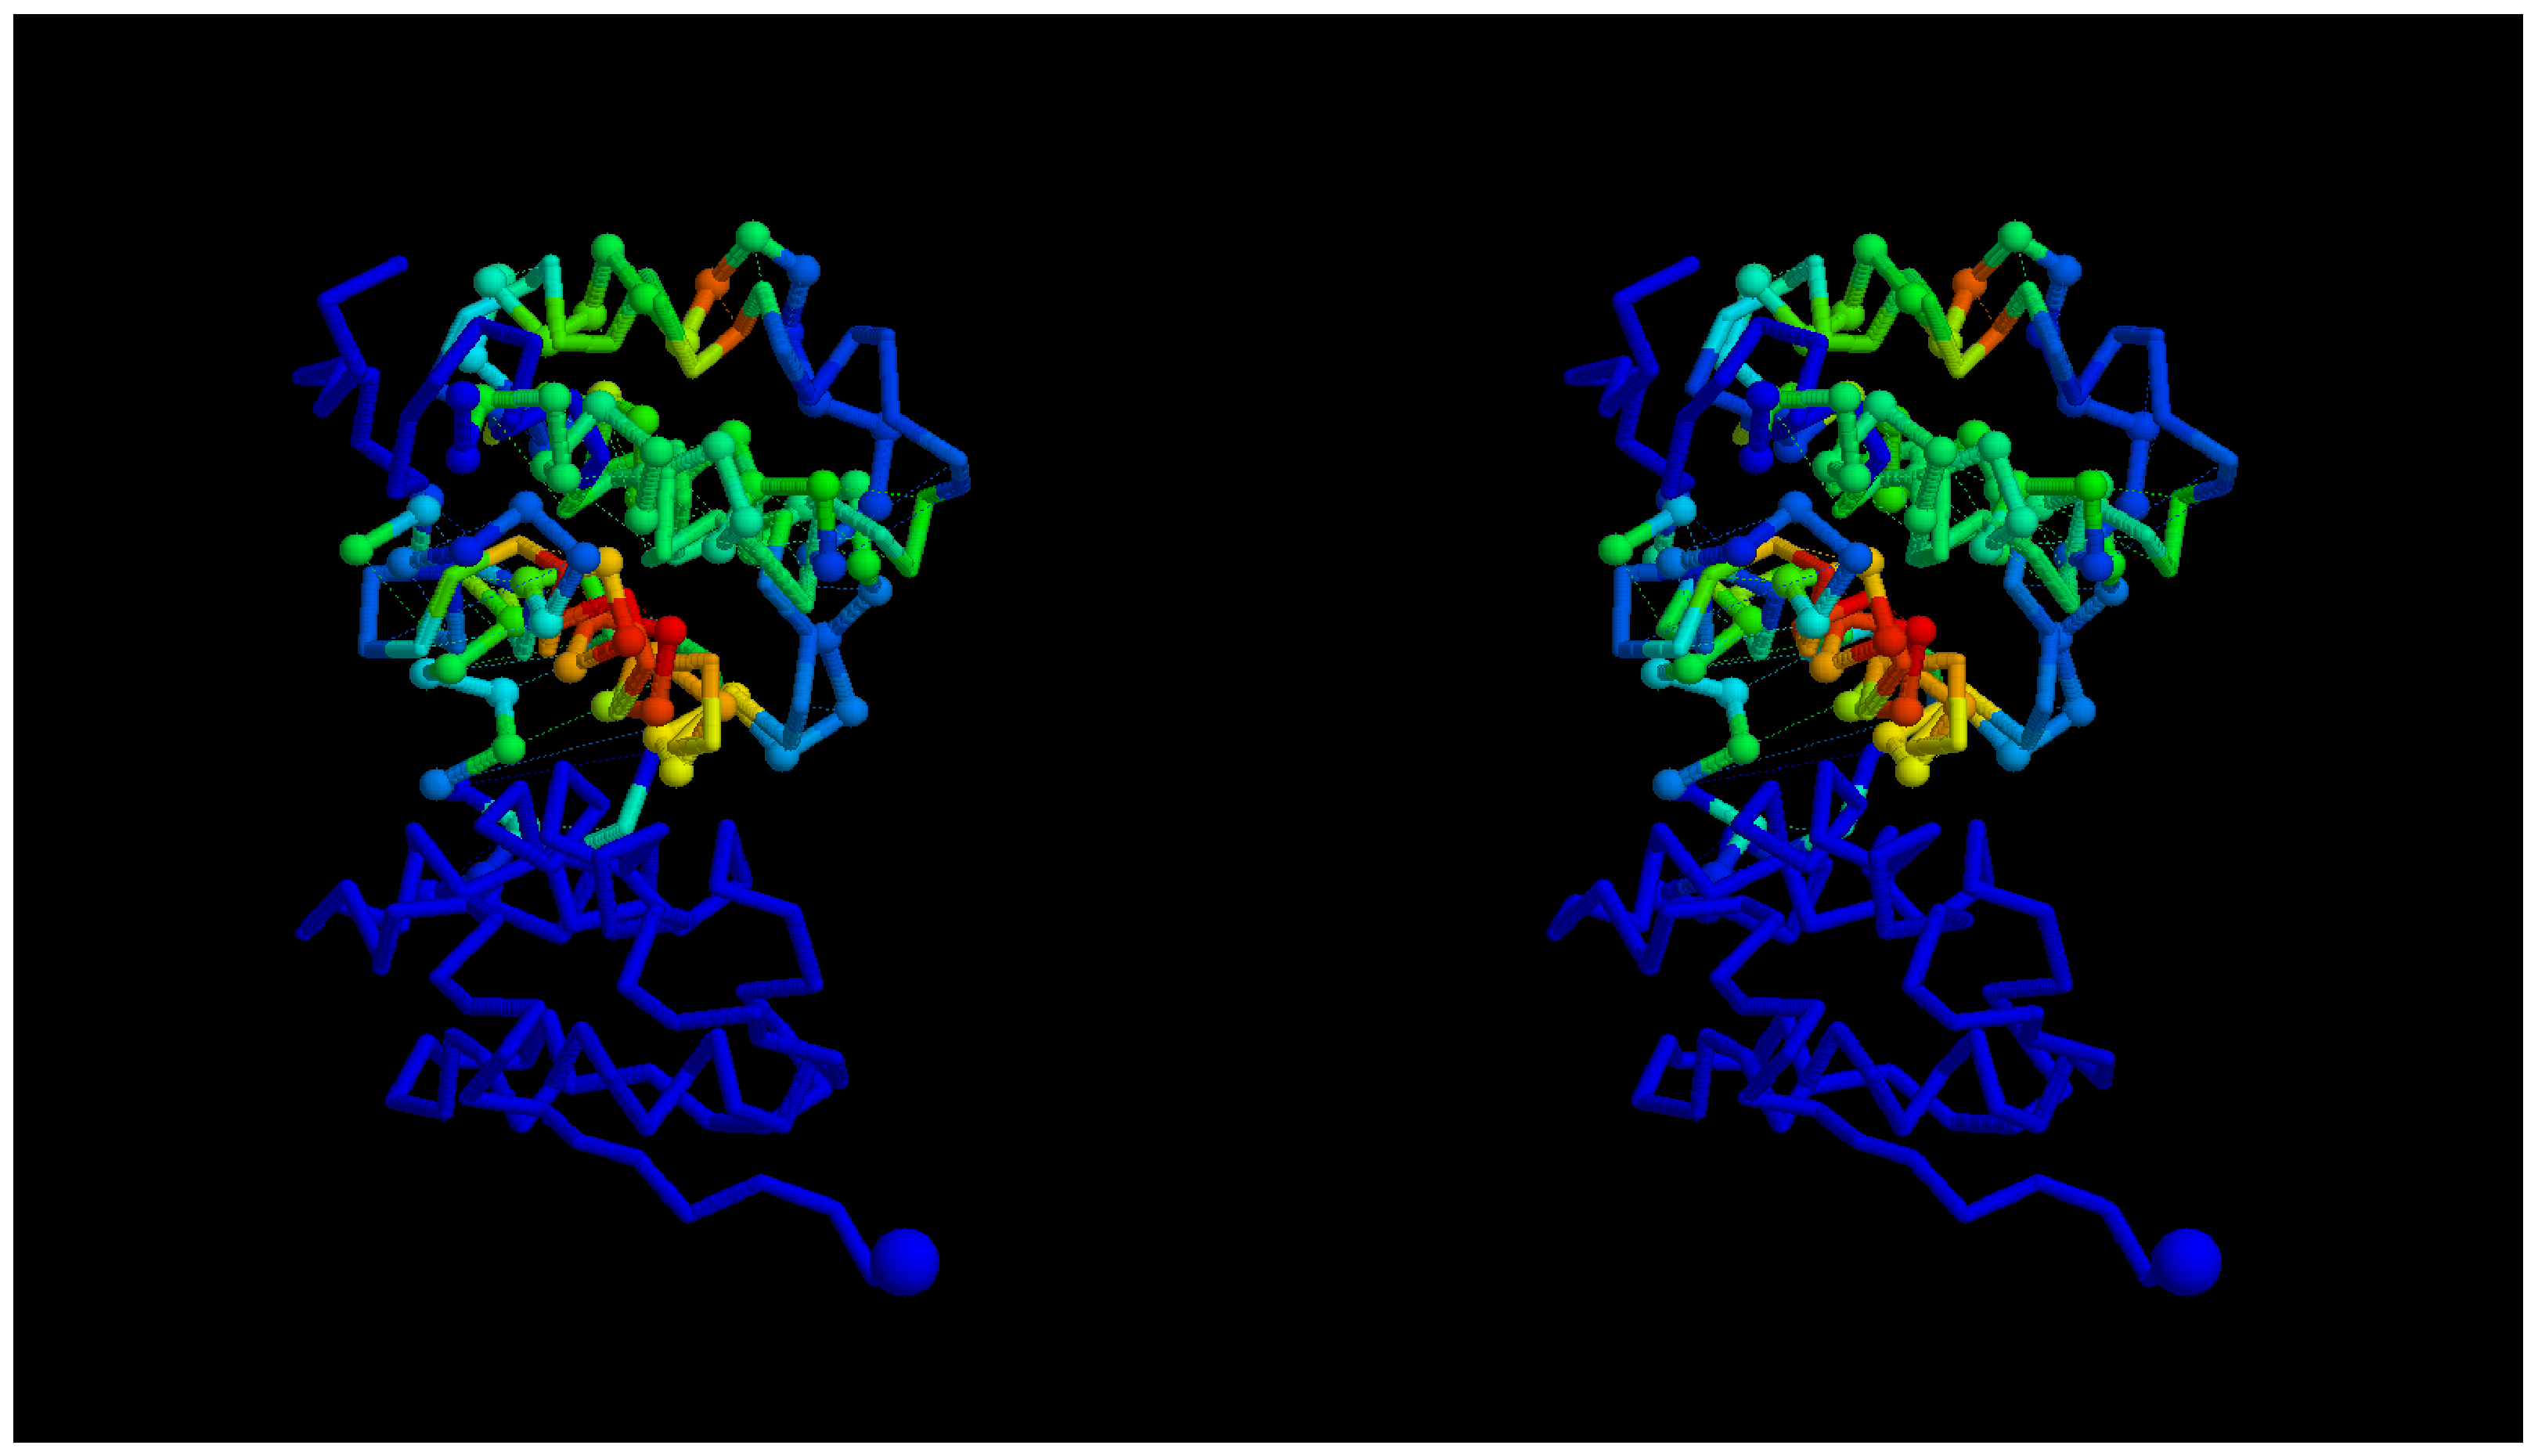
\includegraphics[width=300pt]{full4x3x-super.eps}
}
\subfigure[{\tt 3g29-A}]{
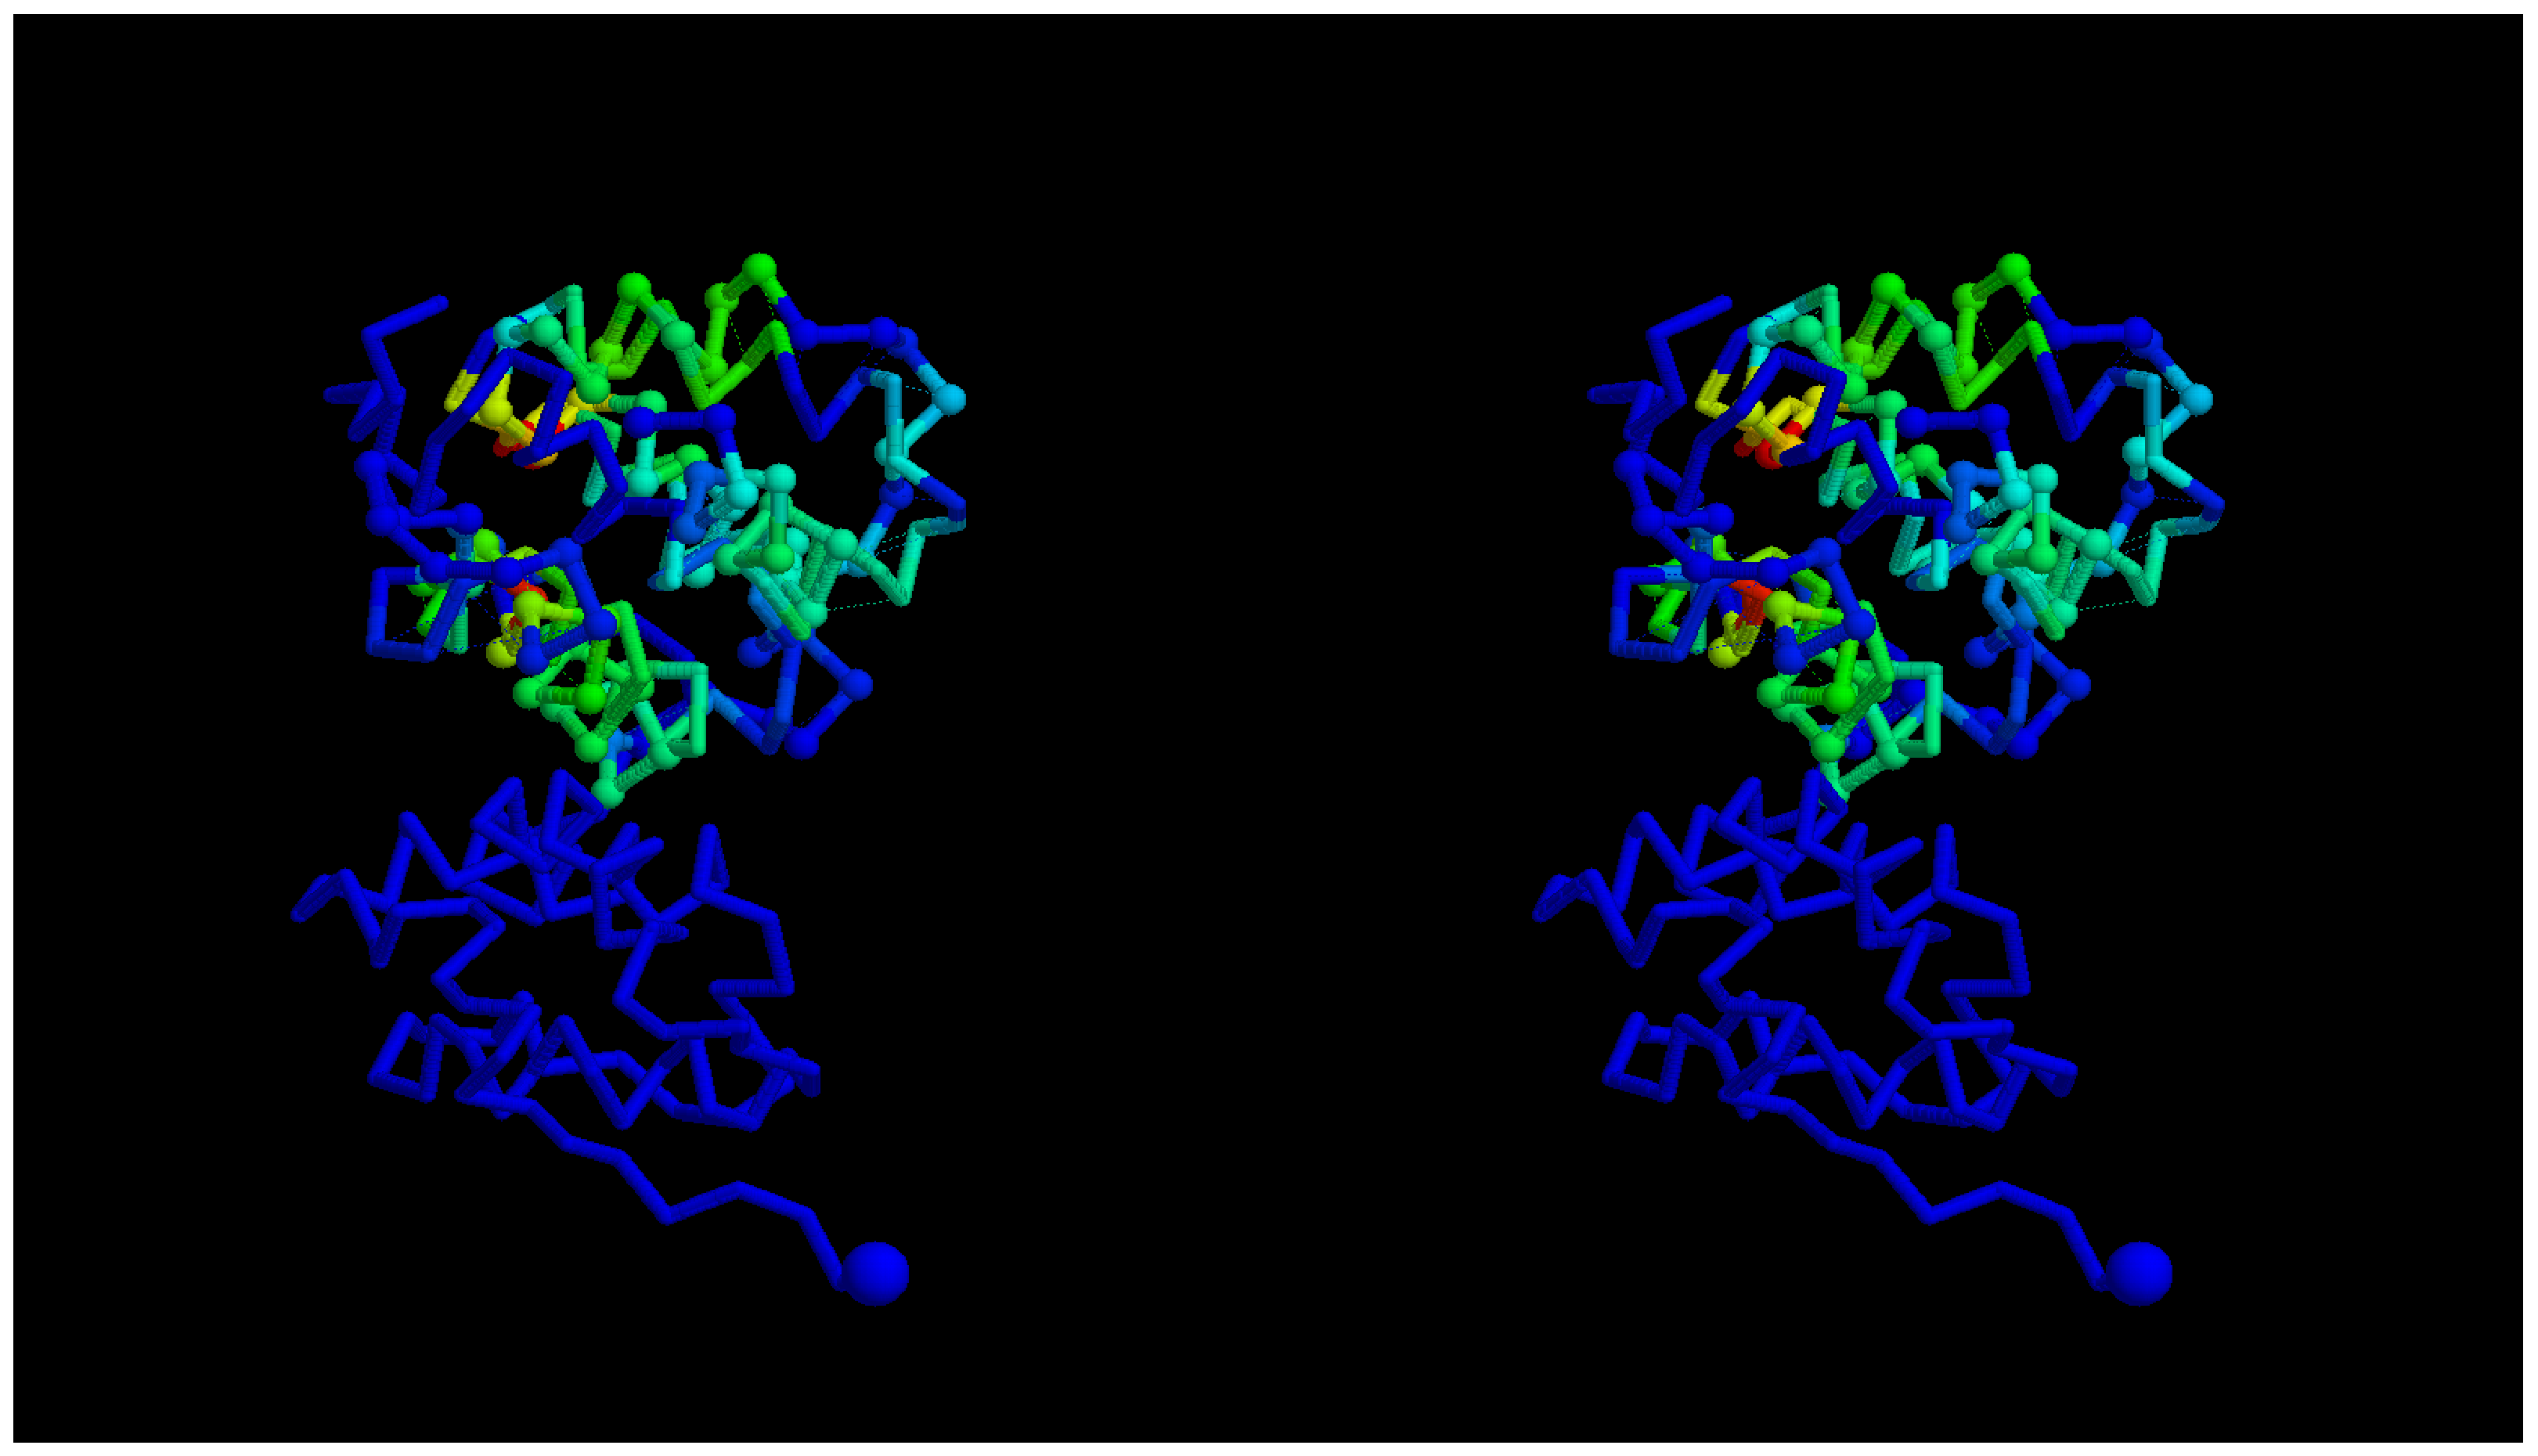
\includegraphics[width=300pt]{full3g29-super.eps}
}
\begin{footnotesize}
\caption{
\label{Fig:top2}
{\bf Top hits superposed}.
The top two \DALI\ hits to the full foamy virus capsid are shown as a \CA\ backbone (stereo pair) coloured using
the residue similarity score calculated by \SAP. (red = strong similarity, blue = none).
The amino terminus of the foamy structure is marked by a large ball and the other structure is distinguished
by small balls on its \CA\ atoms.
($a$) a cytoskeleton associated protein (fragment) of the arc/arg3.1 gene (PDB code: {\tt 4x3x-A}),
(which is thought to have originated from a Ty3/Gypsy retrotransposon family capsid) 
and 
($b$) the structure of the capsid C-terminal domain of the Rous scarcoma virus (PDB code: {\tt 3g29-A}). 
}
\end{footnotesize}
\end{figure}

The result of the DALI search indicated that the Foamy virus structure shares some similarity with the
capsid structure of the ortho-viruses.  However, the matches consist only of a small number of
helices and appears barely more convincing than other matches to proteins that seem very unlikely
to have any meaningful connection to a viral capsid.   The preponderance of capsid matches
throughout the list of hits might seem to add some support to the relationship but may simply be 
a reflection of the number of capsid structures in the structure databank.

Adding confusion to the ortho/foamy relationship is the additional observation that 
the distribution of matches to the ortho-virus structures between the amino (N) and carboxy
(C) terminal domains are mixed.   For example; taking the top 10 matches, the N-terminal domain of the Foamy
structure aligns with 6 C-terminal domains and 4 N-terminal domains of the ortho virsuses
and the best match with the corresponding Foamy C-terminal domain aligns with an ortho N-terminal domain.

%
% Ortho virus: big N, small C
% Foamy smaller N, bigger C
% 
%                  :         :         :         :         |         :         :         :         :         100       :         :         :         :         |         :
% Full    PIGTVIPIQHIRSVTGEPPRNPREIPIWLGRNAPAIDGVFPVTTPDLRCRIINAILGGNIGLSLTPGDCLTWDSAVATLFIRTHGTFPMHQLGNVIKGIVDQEGVATAYTLGMMLSGQNYQLVSGIIRGYLPGQAVVTALQQRLDQEIDNQTRAETFI
% 3g29A-C ---------PWAD--IMQGPS--SFVDFANRLIKAVEGS---ARAPVIIDCFRQKSQPQQLI-------TTPGEIIKYVLDRQ---------------------------------------------------------------------------
% 3g0vA-C ---------PWAD--IMQGPS--SFVDFANRLIKAVEGSAL-ARAPVIIDCFRQKSQPQQLI-------TTPGEIIKYVLDRQ---------------------------------------------------------------------------
% 4ph2A-N RHRAW-ELQDIKK--EIEN----APGSVWIQTLRLAILQADP-TPADLEQLCQYIASPQTAHM-------YQNLWLQAWK-NLPT-------------------------------------------------------------------------
% 3g29B-C ---------PWAD--IMQGPS--SFVDFANRLIKAVEGSNL-ARAPVIIDCFRQKSQPQQLI-------TTPGEIIKYVLDRQ---------------------------------------------------------------------------
% 3g1iB-C ---------PWAD--IMQGPS--SFVDFANRLIKAVEGSDL-ARAPVIIDCFRQKSQPQQLI-------TTPGEIIKYVLDRQ---------------------------------------------------------------------------
% 3g21A-C ---------PWAD--IMQGPS--SFVDFANRLIKAVEGS---ARAPVIIDCFRQKSQPQQLI-------TTPGEIIKYVLDRQ---------------------------------------------------------------------------
% 4ph0C-N RHRAW-ELQDIKKEIENKA-----PGSQWIQTLRLAILQADP-TPADLEQLCQYIASPQTAHM-------YQNLWLQAWKNLPT----------------LQISLADNL----------PDGV--PKEPII-DSLS----------------------
% 4ph0D-N RHRAW-ELQDIKKE-IENK----APGSVWIQTLRLAILQADP-TPADLEQLCQYIASPQTAHM-------YQNLWLQAWKNLP-----------------QISL-ADNL----------PDGV--PKEPIISLSY-----------------------
% 4ph2B-N RHRAW-ELQDIKK--EIEN----APGSVWIQTLRLAILQADP-TPADLEQLCQYIASPQTAHM-------YQNLWLQAWK-NLPT-------------------------------------------------------------------------
% 4cocB-C ---------SILD--IRQGPK--PFRDYVDRFLKTLRAE---VKNWMTETLLVQNANPKTIL-LGPGA-----TLEEMMTACQGVG------------------------------------------------------------------------
% 3g1gB-C ---------PWAD--IMQGPS--SFVDFANRLIKAVEGSDL-ARAPVIIDCFRQKSQPQQLI-------TTPGEIIKYVLDR----------------------------------------------------------------------------
% 1afvB-N ----------------------------------------------------------------------IVQNL-------------SPRTLNAWVKVVEEK-VIPMFSALSE--GATPQDLNTMLNTVGGHQAAMQMLKETINEEASDIAYKRWIILG
% +
% 3nteA-C      YSPTSILD--IRQGPK EPFRDYVDRFYKTLRAEQASQEVKNWMTETLLVQNANPDCKTILKALGPAATLEEMMTACQGV
% 
% PIVQNIQGMVHQAISPRTLNAWVKVVEEKAFSPEVIPMFSALSEGATPQDLNTMLNTVGGHQAAMQMLKETINEEPRGSDIAGTTSTLQEQIGWMTNNPPIPVGEIYKRWIILGLNKIVRM
% ::        : :   : :    :  : :: :   :          :: ::           : :  :   :          :                                 `
% PIISEGNRNRHRAWALRELQDIKKEIENKAPSQVWIQTLRLAIADPTPADLEQLCQYIASQTAHMTSLTAAIAAAEAANTLQGFNPQNGTLTQQSAQPNAGDLRSQYQNLWLQAWKNLPTR
% 
% 
% 4PH2A-N PIISEGN-RNRHRAWALRELQDIKKEIENKAPGSQVWIQTLRLAILQADPTPADLEQLCQYIASPVDQTAHMTSLTAAIAAAEAANTLQGFNPQNGTLTQQSAQPNAGDLRSQYQNLWLQAWKNLPTR
% i                  |                                      || ||  
% 3nteA-N PIVQNIQGQMVHQAISPRTLNAWVKVVEEKAF-SPEVIP--MFSALSEGATPQDLNTMLNTVGGHQAAMQMLKETINEEAAEWDRVHPVHAGPIAPGQMREPRGSDIAGTTSTLQEQIGWMTNNPPIPVGEIYKRWIILGLNKIVRM
%      -C YSPTSILDIRQGPKEPFRDYVDRFYKTLRAEQASQEVKNWMTETLLVQNANPDCKTILKALGPAATLEEMMTACQGV
%
 
\begin{figure}
\centering
\subfigure[Full PDB]{
\label{Fig:daliFULL}
\rotatebox{270}{
\includegraphics[width=140pt]{dali-daliFULL-DALIhitROC.eps}
}}
\subfigure[PDB-90]{
\label{Fig:daliNR90}
\rotatebox{270}{
\includegraphics[width=140pt]{dali-daliNR90-DALIhitROC.eps}
}}
\begin{footnotesize}
\caption{
\label{Fig:rocs}
{\bf PDB capsid structure matches}.
The number of capsid structures identified by the \DALI\ program in ($a$) the full PDB and ($b$)
the 90\% non-redundant PDB (PDB-90) is shown for queries using the full foamy capsid
structure (red), the carboxy terminal domain (green) and the amino terminal domain (blue). 
The number of capsid hits (Y-axis) is plotted against the order of all hits ranked by Z-score
down to a value of 2.   A curve approaching the top left corner indicates greater specificity 
and the extent of a curve to the right indicates the total number of hits.
}
\end{footnotesize}
\end{figure}

\subsubsection{Domain scans}

To clarify the domain match specificity, the two domains of the Foamy virus (1--88 and 89--180,
as defined automatically \cite{TaylorWR99b}) were scanned separately using the \DALI\ program.  
The individual domains were much more specific at matching known capsid structures\footnote{
True/false hits were defined by protein descriptions with the words "CAPSID", "GAG" or "P24".
},   
both in the full PDB and PDB-90 collections as can be seen from the plots in \Fig{rocs}.

The results of these scans strengthened the identification
of the relationship to the ortho capsids and supported the swapped specificity for the N-terminal
match of the Foamy structure with the C-terminal match of the ortho virus and {\em vica versa}, with all
top 12 hits of each domain matching their opposed counterpart.
The structure-based sequence alignments of each domain based on this equivalence are shown in \Fig{swap}.

\begin{figure}
\centering
\begin{singlespace}
\begin{tiny}
\begin{Verbatim}[frame=single]
Nter    PIGTVIPIQHIRSVTGEPPRNPREIPIWLGRNAPAIDGVFPVTTPDLRCRIINAILGGNIGLSLTPGDCLTWDSAVATLFIRTHGTFP
                                :  :: |   |::|        :    ::        :        |    :  :: |      
3g1gA   ---------PWAD--IMQGPS--SFVDFANRLIKAVEGSDL-ARAPVIIDCFRQKSQPQQLI--PSTL-TTPGEIIKYVLDRQK----
3tirA   ---------PWAD--IMQGPS--SFVDFANRLIKAVEGSDL-ARAPVIIDCFRQKSQPQQLI-------TTPGEIIKYVLDRQ-----
3g1iA   ---------PWAD--IMQGPS--SFVDFANRLIKAVEGSDL-ARAPVIIDCFRQKSQPQQLI----TLTT-PGEIIKYVLDRQ-----
3g29A   ---------PWAD--IMQGPS--SFVDFANRLIKAVEGS---ARAPVIIDCFRQKSQPQQLI-------TTPGEIIKYVLDRQ-----
3g0vA   ---------PWAD--IMQGPS--SFVDFANRLIKAVEGSAL-ARAPVIIDCFRQKSQPQQLI-------TTPGEIIKYVLDRQ-----
3g29B   ---------PWAD--IMQGPS--SFVDFANRLIKAVEGSNL-ARAPVIIDCFRQKSQPQQLI-------TTPGEIIKYVLDRQ-----
3g1iB   ---------PWAD--IMQGPS--SFVDFANRLIKAVEGSDL-ARAPVIIDCFRQKSQPQQLI-------TTPGEIIKYVLDRQ-----
3g26A   ---------PWAD--IMQGPS--SFVDFANRLIKAVEGS---CRAPVIIDCFRQKSQPQQLI-------TTPGEIIKYVLDRQ-----
3dtjC   ---------SILD--IRQGPK--EPFRDYVDRFYKTLR--VKNW--MTATLLVQNANPD-TILKGPGA--TLEEMMTA-CQGV-----
3dtjB   ---------SILD--IRQGPK--EPFRDYVDRFYKTLR--VKNW--MTATLLVQNANPD-TILKGPGA--TLEEMMTA-CQGV-----
3dtjA   ---------SILD--IRQGPK--EPFRDYVDRFYKTLR--VKNW--MTATLLVQNANPD-TILKGPGA--TLEEMMTA-CQGV-----
3g21A   ---------PWAD--IMQGPS--SFVDFANRLIKAVEGSDL-ARAPVIIDCFRQKSQPQQLI-------TTPGEIIKYVLDRQ-----

Cter    MHQLGNVIKGIVDQEGVATAYTLGMMLSGQNYQLVSGIIRGYLPGQAVVTALQQRLDQEIDNQTRAETFIQHLNAVYEILGLNARGQSIRL
             |:   :|::   : ::::     |     :  :::     ||:: :|:: :::|:  :     :|  || :  :    
1l6nA   SPRTLNAWVKVVEEKA-IPMFSALSE---GATPDLNTMLNTVGGHQAAMQMLKETINEEA--EIYKRWIILGLNKIVRMYS------PTSI
3j34U   SPRTLNAWVKVVEEKA-IPMFSALSE--GATPQDLNTMLNTVGGHQAAMQMLKETINEEA--EIYKRWIILGLNKIVRMY-------SPTS
4u0bF   SPRTLNAWVKVVEEKA-IPMFSALSC--GATPQDLNTMLNTVGGHQAAMQMLKETINEEA--EIYKRWIILGLNKIVRMY-------SPTS
4u0bG   SPRTLNAWVKVVEEK--IPMFSALSC--GATPQDLNTMLNTVGGHQAAMQMLKETINEEA--EIYKRWIILGLNKIVRMY-------SPTS
3h4eB   SPRTLNAWVKVVEEK--IPMFSALSC--GATPQDLNTMLNTVGGHQAAMQMLKETINEEA--EIYKRWIILGLNKIVRMY-------SPTS
2jprA   SPRTLNAWVKVVEEKA-IPMFSALSE--GATPQDLNTMLNTVGGHQAAMQMLKETINEEA--EIYKRWIILGLNKIVRMY-----------
1afvB   SPRTLNAWVKVVEEKAVIPMFSALSE--GATPQDLNTMLNTVGGHQAAMQMLKETINEEA--EIYKRWIILGLNKIVRMY-------SPTS
4u0bE   SPRTLNAWVKVVEEK--IPMFSALSC--GATPQDLNTMLNTV-GHQAAMQMLKETINEEA--EIYKRWIILGLNKIVRMY-------SPTS
4u0bK   SPRTLNAWVKVVEEK--IPMFSALSC--GATPQDLNTMLNTVGGHQAAMQMLKETINEEA--EIYKRWIILGLNKIVRMY-------SPTS
4u0bH   SPRTLNAWVKVVEEK--IPMFSALSC--GATPQDLNTMLNTVGGHQAAMQMLKETINEEA--EIYKRWIILGLNKIVRMY-------SPTS
2gonA   SPRTLNAWVKVVEEK-VIPXFSALSE--GATPQDLNTXLNTVGGHQAAXQXLKETINEEA--EIYKRWIILGLNKIVRXYS----------
1afvA   SPRTLNAWVKVVEEKAVIPMFSALSE--GATPQDLNTMLNTVGGHQAAMQMLKETINEEA--EIYKRWIILGLNKIVRMY-------SPTS
\end{Verbatim}
\end{tiny}
\end{singlespace}
\begin{footnotesize}
\caption{
\label{Fig:swap}
{\bf Top domain similarity alignments}.
The sequence alignments are shown for the top 12 capsid domain matches found by the \DALI\ program 
using the foamy virus capsid N and C domains separately as a query over the full PDB.
The sequence of the N-terminal domain ({\tt N-ter}) is shown at the top of the first alignment block and the
sequences of the C-terminal domain ({\tt C-ter}) at the top of the second block.   The sequences of the
ortho-virsuses aligned below these all come from the "swapped" relationship of C and N terminal domains,
respectively.   These alignments, which are determined by structure not sequence, exhibit no
specific similarity beyond what would be expected from aligning similar secondary structures from
similar sized domains. (Amino acid identities are marked by a bar and similarities by a colon).
}
\end{footnotesize}
\end{figure}

Although domain transposition is not impossible in viral genomes,  it is sufficiently
unexpected to warrant deeper investigation, especially as it is hard to imagine how an ancestral
capsid protein could tolerate such a large rearrangement and still pack to form a competent shell.
We therefore undertook a more thorougher evaluation using alternative methods to assess the statistical 
significance of these structural similarities.

%
% >3nte
%    Nter PIVQNIQGQMVHQAI
%         SPRTLNAWVKVVEEKAFSPEVIPMFSALSEGATPQDLNTMLNTVGGHQAAMQMLKETINEEAAEWDRVHPVHAGPIAPGQMREPRGSDIAGTTSTLQEQIGWMTNNPPIPVGEIYKRWIILGLNKIVRM
%    Cter YSPTSILDIRQGPKEPFRDYVDRFYKTLRAEQASQEVKNWMTETLLVQNANPDCKTILKALGPAATLEEMMTACQGV
% wtaylor@wt:~/ianpdbs/dali$ cut -c 6-175 newN.aln | head -14
%                  :         :         :         :         |         :         :         :        
% Nter    PIGTVIPIQHIRSVTGEPPRNPREIPIWLGRNAPAIDGVFPVTTPDLRCRIINAILGGNIGLSLTPGDCLTWDSAVATLFIRTHGTFP
% 3g1gA   ---------PWAD--IMQGPS--SFVDFANRLIKAVEGSDL-ARAPVIIDCFRQKSQPQQLI--PSTL-TTPGEIIKYVLDRQK----
% 3tirA   ---------PWAD--IMQGPS--SFVDFANRLIKAVEGSDL-ARAPVIIDCFRQKSQPQQLI-------TTPGEIIKYVLDRQ-----
% 3g1iA   ---------PWAD--IMQGPS--SFVDFANRLIKAVEGSDL-ARAPVIIDCFRQKSQPQQLI----TLTT-PGEIIKYVLDRQ-----
% 3g29A   ---------PWAD--IMQGPS--SFVDFANRLIKAVEGS---ARAPVIIDCFRQKSQPQQLI-------TTPGEIIKYVLDRQ-----
% 3g0vA   ---------PWAD--IMQGPS--SFVDFANRLIKAVEGSAL-ARAPVIIDCFRQKSQPQQLI-------TTPGEIIKYVLDRQ-----
% 3g29B   ---------PWAD--IMQGPS--SFVDFANRLIKAVEGSNL-ARAPVIIDCFRQKSQPQQLI-------TTPGEIIKYVLDRQ-----
% 3g1iB   ---------PWAD--IMQGPS--SFVDFANRLIKAVEGSDL-ARAPVIIDCFRQKSQPQQLI-------TTPGEIIKYVLDRQ-----
% 3g26A   ---------PWAD--IMQGPS--SFVDFANRLIKAVEGS---CRAPVIIDCFRQKSQPQQLI-------TTPGEIIKYVLDRQ-----
% 3dtjC   ---------SILD--IRQGPK--EPFRDYVDRFYKTLR--VKNW--MTATLLVQNANPD-TILKGPGA--TLEEMMTA-CQGV-----
% 3dtjB   ---------SILD--IRQGPK--EPFRDYVDRFYKTLR--VKNW--MTATLLVQNANPD-TILKGPGA--TLEEMMTA-CQGV-----
% 3dtjA   ---------SILD--IRQGPK--EPFRDYVDRFYKTLR--VKNW--MTATLLVQNANPD-TILKGPGA--TLEEMMTA-CQGV-----
% 3g21A   ---------PWAD--IMQGPS--SFVDFANRLIKAVEGSDL-ARAPVIIDCFRQKSQPQQLI-------TTPGEIIKYVLDRQ-----
% +
% 3nteA-C      YSPTSILD--IRQGPK--EPFRDYVDRFYKTLRaeqasqeVKNWMTETLLVQNANPDckTILKALGPAaTLEEMMTACQGV
% 
%      -N PIVQNIQGQMVHQAISPRTLNAWVKVVEEKAFSPEVIPMFSALSEGATPQDLNTMLNTVGGHQAAMQMLKETINEEAAEWDRVHPVHAGPIAPGQMREPRGSDIAGTTSTLQEQIGWMTNNPPIPVGEIYKRWIILGLNKIVRM
% 3nteA-C YSPTSILDIRQGPKEPFRDYVDRFYKTLRAEQASQEVKNWMTETLLVQNANPDCKTILKALGPAATLEEMMTACQGV
% 
% wtaylor@wt:~/ianpdbs/dali$ cut -c 6-175 newC.aln | head -14
%                  :         :         :         :         |         :         :         :         :  
% Cter    MHQLGNVIKGIVDQEGVATAYTLGMMLSGQNYQLVSGIIRGYLPGQAVVTALQQRLDQEIDNQTRAETFIQHLNAVYEILGLNARGQSIRL
% 1l6nA   SPRTLNAWVKVVEEKA-IPMFSALSE---GATPDLNTMLNTVGGHQAAMQMLKETINEEA--EIYKRWIILGLNKIVRMYS------PTSI
% 3j34U   SPRTLNAWVKVVEEKA-IPMFSALSE--GATPQDLNTMLNTVGGHQAAMQMLKETINEEA--EIYKRWIILGLNKIVRMY-------SPTS
% 4u0bF   SPRTLNAWVKVVEEKA-IPMFSALSC--GATPQDLNTMLNTVGGHQAAMQMLKETINEEA--EIYKRWIILGLNKIVRMY-------SPTS
% 4u0bG   SPRTLNAWVKVVEEK--IPMFSALSC--GATPQDLNTMLNTVGGHQAAMQMLKETINEEA--EIYKRWIILGLNKIVRMY-------SPTS
% 3h4eB   SPRTLNAWVKVVEEK--IPMFSALSC--GATPQDLNTMLNTVGGHQAAMQMLKETINEEA--EIYKRWIILGLNKIVRMY-------SPTS
% 2jprA   SPRTLNAWVKVVEEKA-IPMFSALSE--GATPQDLNTMLNTVGGHQAAMQMLKETINEEA--EIYKRWIILGLNKIVRMY-----------
% 1afvB   SPRTLNAWVKVVEEKAVIPMFSALSE--GATPQDLNTMLNTVGGHQAAMQMLKETINEEA--EIYKRWIILGLNKIVRMY-------SPTS
% 4u0bE   SPRTLNAWVKVVEEK--IPMFSALSC--GATPQDLNTMLNTV-GHQAAMQMLKETINEEA--EIYKRWIILGLNKIVRMY-------SPTS
% 4u0bK   SPRTLNAWVKVVEEK--IPMFSALSC--GATPQDLNTMLNTVGGHQAAMQMLKETINEEA--EIYKRWIILGLNKIVRMY-------SPTS
% 4u0bH   SPRTLNAWVKVVEEK--IPMFSALSC--GATPQDLNTMLNTVGGHQAAMQMLKETINEEA--EIYKRWIILGLNKIVRMY-------SPTS
% 2gonA   SPRTLNAWVKVVEEK-VIPXFSALSE--GATPQDLNTXLNTVGGHQAAXQXLKETINEEA--EIYKRWIILGLNKIVRXYS----------
% 1afvA   SPRTLNAWVKVVEEKAVIPMFSALSE--GATPQDLNTMLNTVGGHQAAMQMLKETINEEA--EIYKRWIILGLNKIVRMY-------SPTS
% +
% 3nteA-N SPRTLNAWVKVVEEKAFSPEVIPMFSALSEGATPQDLNTMLNTVGGHQAAMQMLKETINEEAAEWDRVHPVHAGPIAPGQMREPRGSDIAGTTSTLQEQIGWMTNNPPIPVGEIYKRWIILGLNKIVRM
% 
% 3nteA-N PIVQNIQGQMVHQAI
%         SPRTLNAWVKVVEEKAFSPEVIPMFSALSEGATPQDLNTMLNTVGGHQAAMQMLKETINEEAAEWDRVHPVHAGPIAPGQMREPRGSDIAGTTSTLQEQIGWMTNNPPIPVGEIYKRWIILGLNKIVRM
%      -C YSPTSILDIRQGPKEPFRDYVDRFYKTLRAEQASQEVKNWMTETLLVQNANPDCKTILKALGPAATLEEMMTACQGV
% 

\subsection{Structural alignment significance}

\subsubsection{Reversed-structure searches}

For each comparison, the DALI program calculates an empirical Z-score, combining an estimation of
significance with protein length normalisation.   The program reports all matches over Z=2, however,
when the proteins are small and especially when the structures being compared are both predominantly
alpha-helical in nature, then matches over this cutoff include many functionally unrelated
hits where the similarity has arisen through the fortuitous alignment of a few helices.

Therefore, to calculate a stricter cutoff on score, we created a decoy probe by reversing the
alpha-carbon backbone then reconstructing the full atomic structure, using a simple algorithm
to regenerate a full backbone\footnote{
Note that reversing the \CA\ backbone does not change the chirality of the \A-helices
but as \DALI\ requires a full atomic backbone, this must be restored on the reversed chain.
}).
\Fig{revs} plots the ranked DALI Z-scores for the separate (native) foamy domains.
% N red=T, cyan=F: C magenta=T, green=F
As would be expected, the larger C-terminal domain has hits with a higher significance than the
smaller N-terminal domain:  the former covers the range Z=2.5 to Z=5 over the true hits (magenta
dots) whereas the latter tracks a similar profile running one Z-value unit lower (2--4 over true
red dots).  Plotting the Z-scores against the log of their rank produces almost linear traces
for the hits from the PDB-90, making it easy to compare N-domain (red/cyan dots) with C-domain 
(magenta/green dots) (for T/F hits) in \Fig{revs}.

The equivalent scans with the reversed domain structures, using both the foamy and ortho (HIV) structures 
(neither of which should have any particular relationship to the capsid or any other natural protein)
also found hits with high Z-scores (black and blue points in \Fig{revs}, respectively).
When compared with the native domains (\Fig{revs}), these decoys had a profile that tracked mostly above
the N-terminal native domain but below the C-terminal domain.  However, with the latter domain, this
was only distinct in the hits to the full PDB whereas with the PDB-90, the native domain was only clearly 
better over the top 10 matches, half of which were to non-capsid structures.

% set style line  1 lt rgb "black"
% set style line  2 lt rgb "red" 
% set style line  3 lt rgb "cyan"
% set style line  4 lt rgb "magenta"
% set style line  5 lt rgb "green"
% set style line  6 lt rgb "blue"
% plot [-0.1:][1.9:5.1]\
% '3etnN.dat' u (log($1)):(($3-0.04))    ls 6  pt 7 ps 0.7 not, \
% '3etnC.dat' u (log($1)):(($3-0.04))    ls 6  pt 5 ps 0.7 not, \
% 'wenN.dat' u (log($1)):(($3-0.02))     ls 1  pt 7 ps 0.7 not, \
% 'wenC.dat' u (log($1)):(($3-0.02))     ls 1  pt 5 ps 0.7 not, \
% 'capFnewN.dat' u (log($2)):(($4))      ls 3  pt 7 ps 0.7 not, \
% 'capTnewN.dat' u (log($2)):(($4+0.02)) ls 2  pt 7 ps 0.7 not, \
% 'capFnewC.dat' u (log($2)):(($4))      ls 5  pt 7 ps 0.7 not, \
% 'capTnewC.dat' u (log($2)):(($4+0.02)) ls 4  pt 7 ps 0.7 not
% set terminal postscript color
% set output 'rawDALIdom.ps'
 
\begin{figure}
\centering
\subfigure[full PDB]{
\label{Fig:daliNR90}
\rotatebox{270}{
\includegraphics[width=140pt]{dali-daliFULL-rawDALIdom.eps}
}}
\subfigure[PDB-90]{
\label{Fig:daliFULL}
\rotatebox{270}{
\includegraphics[width=140pt]{dali-daliNR90-rawDALIdom.eps}
}}
\begin{footnotesize}
\caption{
\label{Fig:revs}
{\bf Ranked \DALI\ scores with decoys}.
The \DALI\ Z-scores (Y-axis) are plotted against the log$_{10}$ of their ranked position in the 
list of hits (X-axis) with the amino-terminal domain (N) as T=red, F=cyan dots and the carboxy-terminal domain (C)
as T=magenta and F=green dots, where T is a true capsid hit and F is a false hit to a non-capsid protein.
Four sets of decoys are compared to these, consisting of the reversed foamy capsid domains in
black and the reversed HIV capsid domains in dark-blue (with a circle = N and a square = C domains in both).
The \DALI\ score for each set of hits has been slightly displaced to prevent coincident dots from being
obscured.  (This happens because of the integral number of residues and the \DALI\ score being specified
to only one decimal place).
}
\end{footnotesize}
\end{figure}

The results with the simple reversed decoy using \DALI\, suggested that the match of the foamy virus domains to the
ortho virus capsid N-terminal domain may be due to chance and that the match to the C-terminal domain looks 
meaningful if based on the hits to the full PDB but may be only marginal based on the PDB-90 hits. 

However, both the N and C terminal domains pocess a degree of internal symmetry which gives
rise to a partial match with their reversed 'doppleganger' decoys.   The N-terminal domain superposed on its decoy
had an RMSD of 5.4/60 (\AA/\CA s) and 5.5/24 for the C-terminal domain.   The higher symmetry of the smaller
domain may be sufficient to explain its poor level of specificity seen in \Fig{revs} and to try and resolve this
ambiguity, a more diverse set of decoys were generated based on cyclic permutation and segment swapping combined
with chain reversal \cite{TaylorWR06a}.

\begin{figure}
\centering
\subfigure[N]{
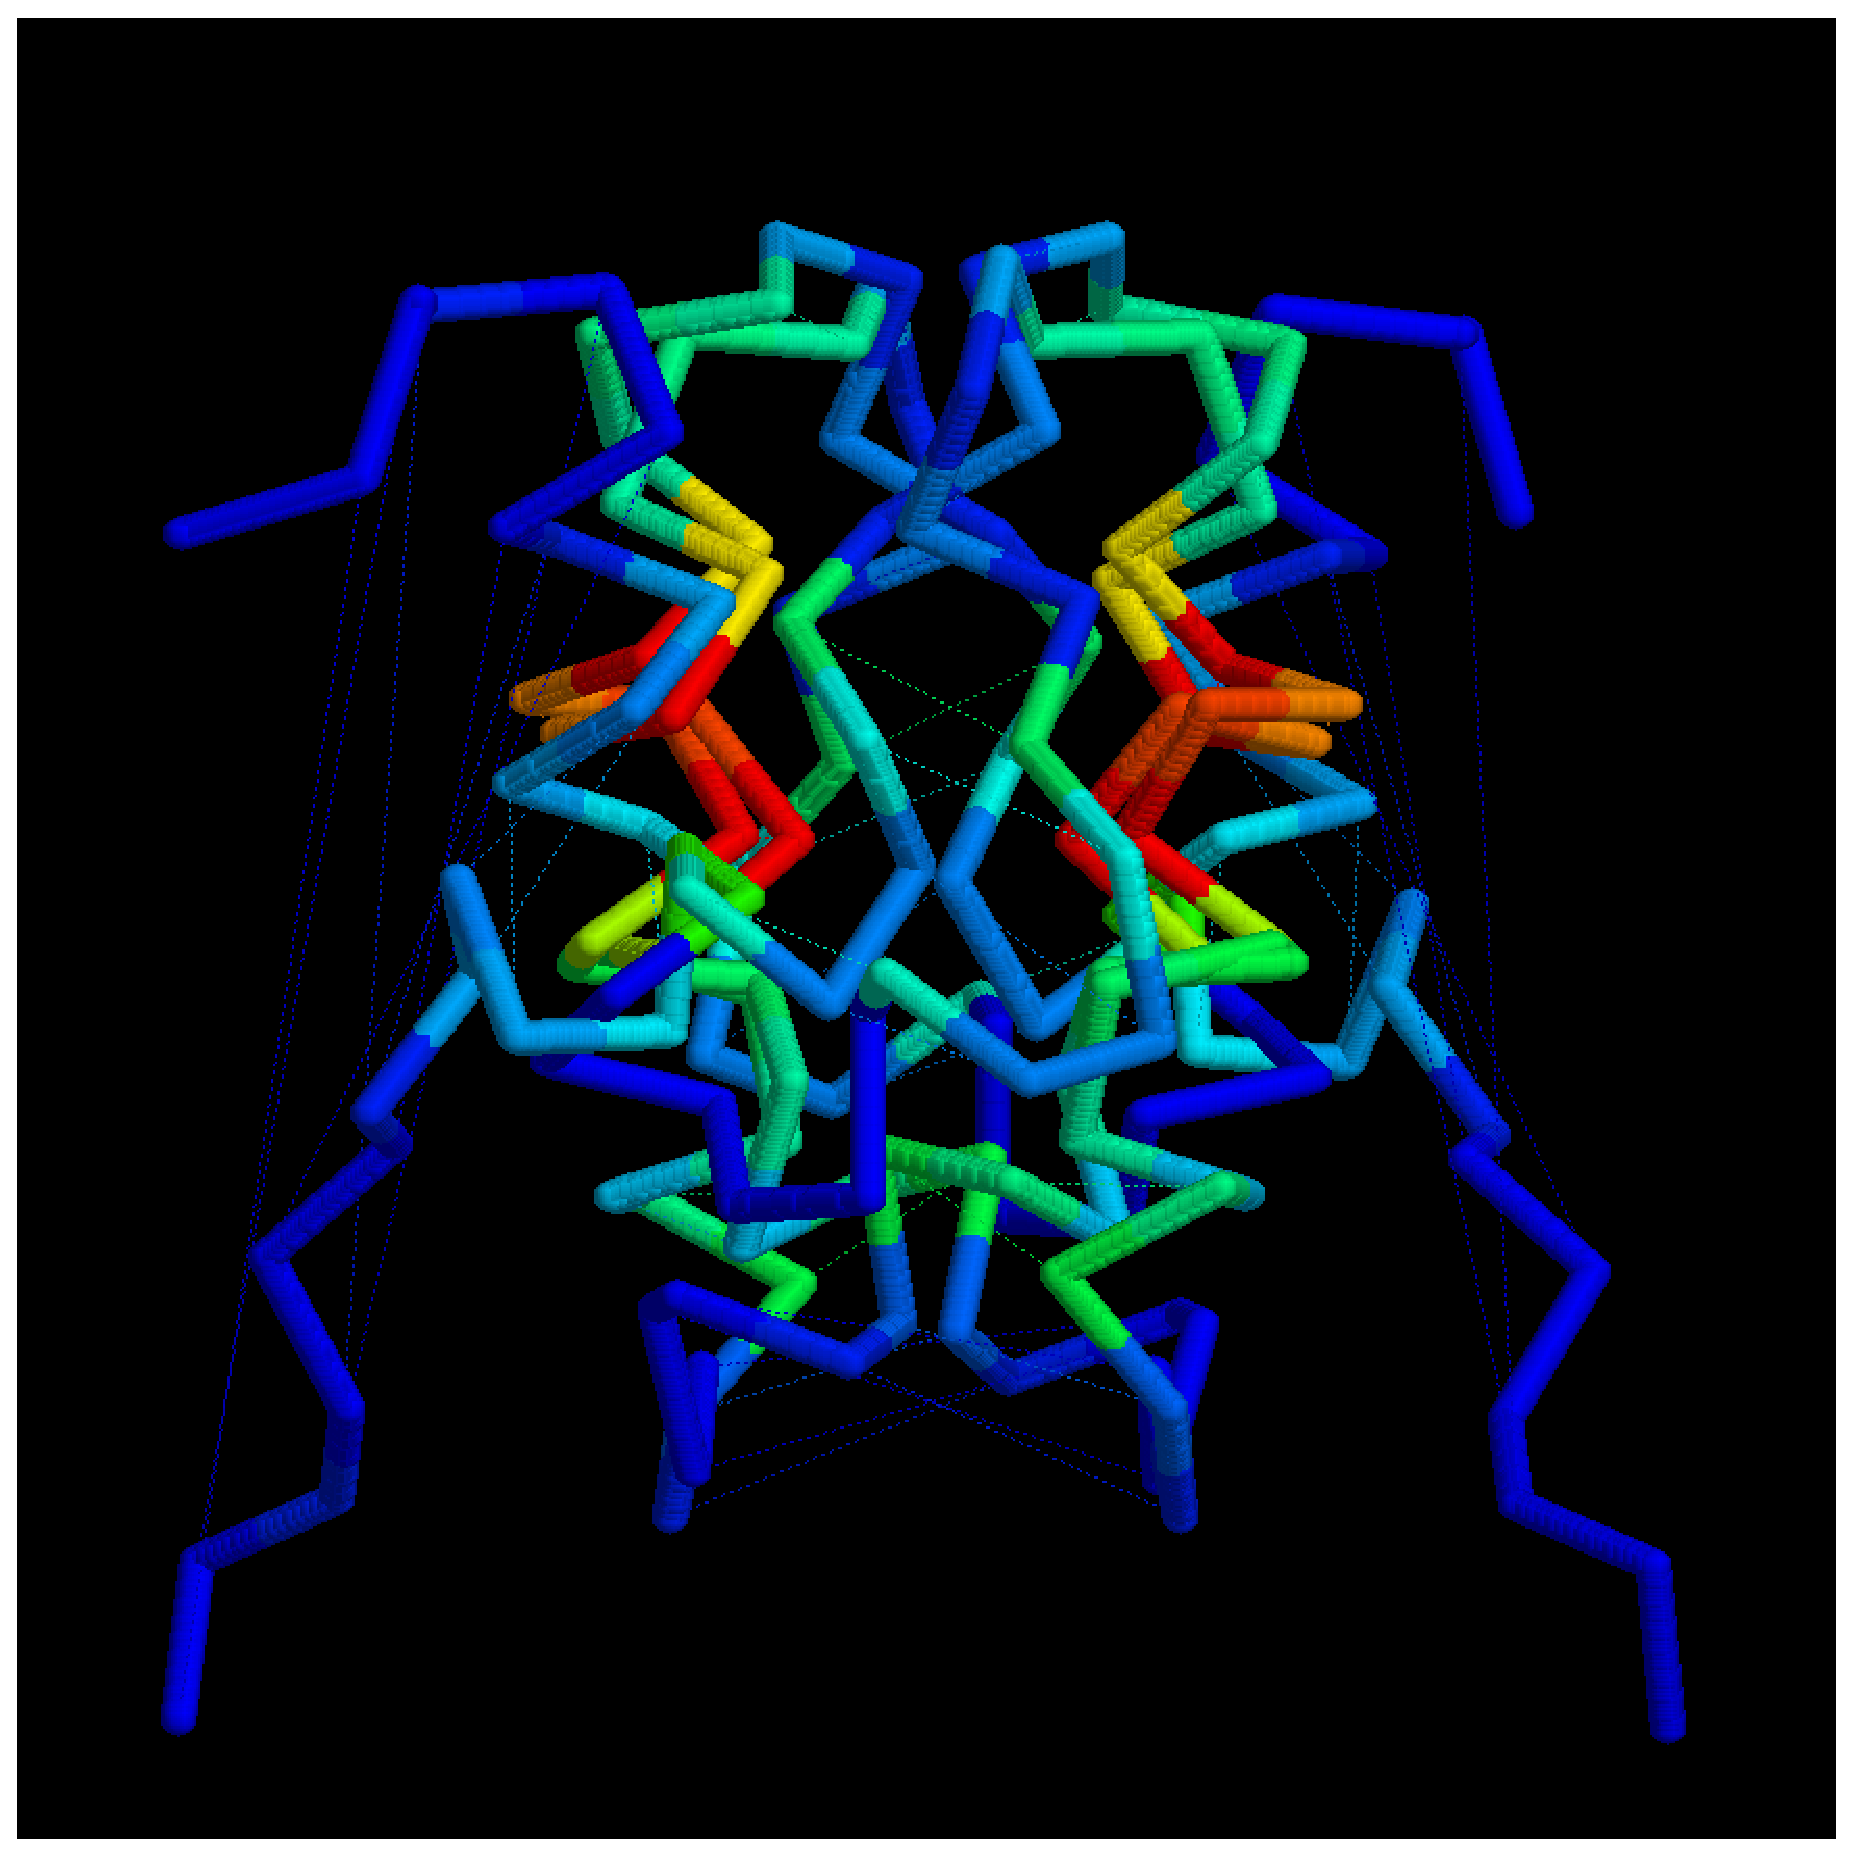
\includegraphics[width=150pt]{twoN.eps}
}
\subfigure[C]{
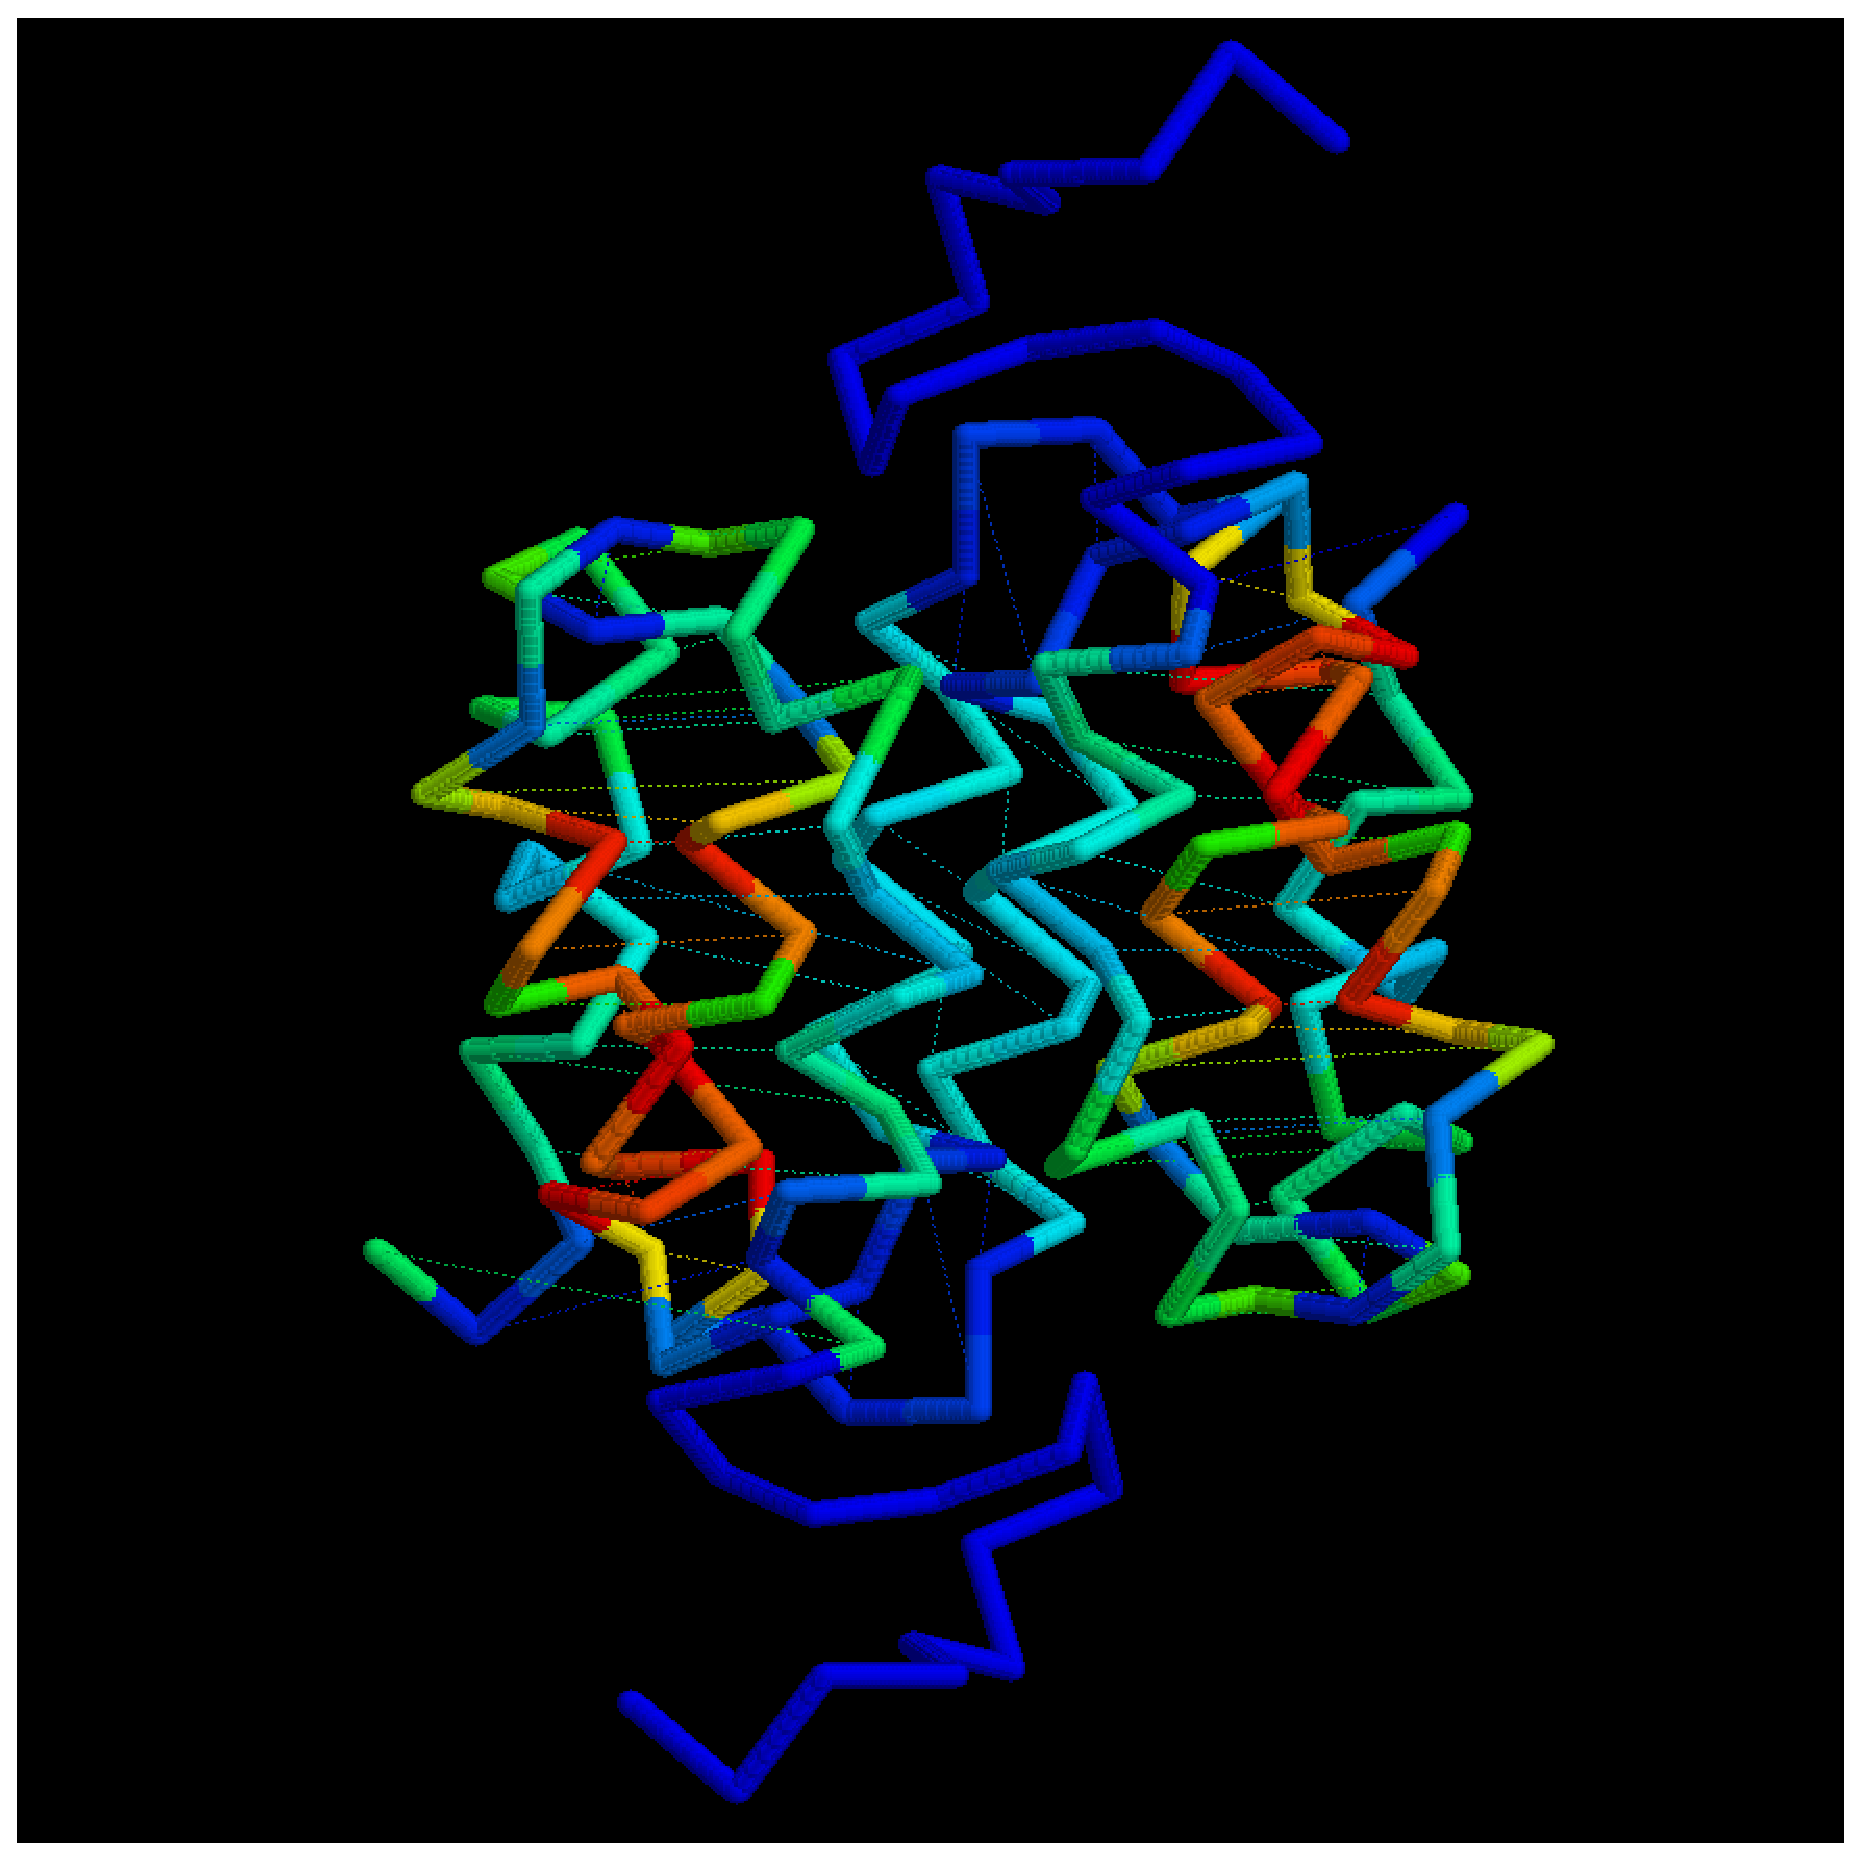
\includegraphics[width=150pt]{twoC.eps}
}
\begin{footnotesize}
\caption{
\label{Fig:tows}
{\bf Native/decoy similarity}.
When superposed using the program \SAP, both N-terminal (left) and C-terminal (right) domains
have some degree of similarity to their reversed decoy 'doppleganger', which is more marked
for the N domain.   The superposed structures are coloured by the \SAP\ residue-level score as
red = high similarity, blue = low.  The N domain has roughly 60 equivalent \CA\ positions
compared to only 24 in the larger C domain.
}
\end{footnotesize}
\end{figure}

\subsubsection{Customised decoy comparisons}

To improve the statistical analysis of the foamy/ortho capsid similarity, we employed a method
based on the generation of a population of customised 'decoy' models to provide a background distribution
of unrelated protein scores \cite{TaylorWR06a}.  This method retains the advantage of the simple
reversed structures where every comparison that constitutes the random pool is between two models
of the same size and secondary structure composition as the pair of native structures being compared.
For this study we collected 12 capsid N-terminal domains and 7 C-terminal domains, each of which 
were compared with the foamy N-terminal domain and the foamy C-terminal domain.
(The structures are identified in Table 1 with full details in the Methods section).

For each domain pair to be compared, decoys were created using cyclic permutation and segment
swapping with chain reversal to generate a family of customised decoys for each comparison
\cite{TaylorWR06a}.  All pairs of forward/reversed decoys were then compared, with each pair being
drawn from a pool of models generated from the two native structures.  This ensures that the native
domains (which may have different lengths) are always evaluated against a decoy pair with the same
length combination.   (See Methods section for details).   All the decoy comparisons, of which
there are typically 150--300 for each comparison,  can then be compared to the native pair on a
plot of RMSD against the number of matched residues (\CA\ atoms).   An example is shown in
\Fig{sapit} for the comparison of the HIV1 structure (PDB codes: 1ak4 (N) and 1a43 (C)) domains
against the foamy virus gag domains.
 
\begin{figure}
\centering
\subfigure[orthoN+foamyN]{
\label{Fig:sapitNN}
\rotatebox{270}{
\includegraphics[width=140pt]{sapitNN.eps}
}}
\subfigure[orthoN+foamyC]{
\label{Fig:sapitNC}
\rotatebox{270}{
\includegraphics[width=140pt]{sapitNC.eps}
}}
\subfigure[orthoC+foamyN]{
\label{Fig:sapitCN}
\rotatebox{270}{
\includegraphics[width=140pt]{sapitCN.eps}
}}
\subfigure[orthoC+foamyC]{
\label{Fig:sapitCC}
\rotatebox{270}{
\includegraphics[width=140pt]{sapitCC.eps}
}}
\begin{footnotesize}
\caption{
\label{Fig:sapit}
{\bf ortho/foamy domains compared with customised decoys}.
Each amino (N), carboxy (C) domain combination between the ortho retrovirus capsid structure (HIV1)
and the foamy virus capsid structure is plotted as a line for increasingly large subsets of matched
positions against their RMSD (Y-axis), as in Figure 2.  The point on this line marks the lowest
$a$-value (\Eqn{fit}), however, to be consistent with the decoy data, the full alignment length
was used.  The decoy comparison data (blue) is plotted in a variety of symbols
with each representing a different combination of decoy construction.  The dashed blue lines
(which are the same in all plots) mark the approximate 10$^{th}$ percentile boundaries of
the decoy generated distributions,  with {\tt a} = 1.7 (upper) and  {\tt a} = 0.8 (lower). 
(See Methods section for details).
}
\end{footnotesize}
\end{figure}

\begin{figure}
\centering
\subfigure[]{
\label{Fig:normHIV}
\rotatebox{270}{
\includegraphics[width=140pt]{fitsCN-plothiv.eps}
}}
\subfigure[]{
\label{Fig:normALL}
\rotatebox{270}{
\includegraphics[width=140pt]{fitsCN-plotall.eps}
}}
\begin{footnotesize}
\caption{
\label{Fig:norms}
{\bf ortho-C and foamy-N domain comparison statistics}.
The $a$-value (normalised RMSD) for the comparison of the ortho-C and foamy-N decoy domains
(Figure 8($b$)) are plotted as a frequency distribution (red) along with a bell-shaped
Normal distribution curve (green) with matching mean ($\mu$) and spread ($\sigma$).
Part ($a$) shows the distribution for the HIV1 C-terminal domain ($\mu = 1.23$) and spread ($\sigma = 0.17$)
with the position of the native structure comparison plotted as a blue (inverted) triangle.  
Its position lies 0.64 units below the mean giving a Z-score of $0.64/0.17 = 3.76$.
Part ($b$) shows the combined data from seven representative viruses (in Table 1).
These data comprise two distributions, that of the combined decoys and also the much smaller
distribution of native scores (blue triangles).   This allows a T-test to be made on the
significance of their separation.
}
\end{footnotesize}
\end{figure}

%
%  Run sapit.csh for each domain against the foamy N and C
%
%wtaylor@wt:~/ianpdbs/sapit$ cat rundom.csh
%# 1 = domain
%
%mkdir $argv[1]
%cd $argv[1]
%ln -s ~/util
%ln -s ~/sapit main
%ln -s .. home
%ln -s ../pdb
%tcsh main/sapit.csh $argv[1] foamN > $argv[1]N.log
%tcsh main/sapit.csh $argv[1] foamC > $argv[1]C.log
%
% and do this for each capsid domain
%
%wtaylor@wt:~/ianpdbs/sapit$ cat rundoms.csh
%foreach dom (`cat [NC]term.list`)
%	echo $dom
%	tcsh rundom.csh $dom
%end
%
% convert the comparisons into Z-scores using sapit/fits1.c
% fits1 reads the true and the random scores and discards
% random pairs outside +/-10 of the true alignment length.
% It then converts the RMS:Length (r:x) values into... 
% a[i] = r/(sqrt(x)*(1-exp(-x*x/damp)));
% The mean and std. of a[] give the Z-score for the true.
%
% NB the values of margin = 10 and damp = 30 were used
%
%wtaylor@wt:~/ianpdbs/sapit$ more scoreZ.csh
%rm score*.dat
%set foamN = `echo foamN`
%set foamC = `echo foamC`
%foreach dom (`cat Nterm.list`)
%	echo $dom
%	set score = `main/fits1 $dom/$dom$foamN` 
%	echo $dom+N $score >> scoreNN.dat
%	set score = `main/fits1 $dom/$dom$foamC` 
%	echo $dom+C $score >> scoreNC.dat
%end
%foreach dom (`cat Cterm.list`)
%	echo $dom
%	set score = `main/fits1 $dom/$dom$foamN` 
%	echo $dom+N $score >> scoreCN.dat
%	set score = `main/fits1 $dom/$dom$foamC` 
%	echo $dom+C $score >> scoreCC.dat
%end
%
% NB now : main/fits1 $dom/$dom$foamC 10 30.0
% for 4x3x (ARC protein)
%wtaylor@wt:~/ianpdbs/sapit$ main/fits1 4x3x/4x3xfoamN 10 30.0
% damp = 10.000000 margin = 30
% n = 190 mean = 1.278401 stdv = 0.207008 y = 0.670932 mean-y = 0.607469 z = 2.934513
%wtaylor@wt:~/ianpdbs/sapit$ main/fits1 4x3x/4x3xfoamC 10 30.0
% damp = 10.000000 margin = 30
% n = 213 mean = 1.253246 stdv = 0.262764 y = 0.589290 mean-y = 0.663956 z = 2.526810


\subsubsection{Statistical analysis of the decoy comparisons}

The quality of the comparisons in \Fig{sapit} can be quantified as a combination of their
RMSD ($R$) and the number of matched (superposed) positions ($N$).   However, as explained in 
the Methods section, for statistical analysis, it is easier to combine this pair of numbers
as a single number,  called the $a$-value (\Eqn{fit}), which is the scaling factor that
causes a theoretical curve to pass through the point ($R,N$).

When expressed by a single $a$-value
all the data points in a comparison, such as \Fig{sapitCN},
can be plotted as a frequency histogram and examined to see if they approximate a Normal
distribution.   The distributions were found to be a good fit to unskewed Gaussians and
so were treated as normal distributions (rather than extreme value distributions
that have also been considered previously as a model for random structure comparison scores
\cite{LevittMet98,TaylorWR06a}).    The frequency data from the comparison of the orthoN domain from
HIV1 and the foamyC domain (\Fig{sapitCN}) is shown in \Fig{normHIV} along with a Normal  
distribution that has the same mean ($\mu$) and standard deviation ($\sigma$) as the data.
On this plot, the value of $a$ (\Eqn{fit}) for the comparison of the
native pair of domains is also plotted (blue triangle) and from its position, a Z-score
can be calculated.

In this way, the significance of all combinations of the native ortho and foamy domain
superpositions were calculated, using the background distribution of 'customised' decoy
comparisons based on each individual native pair.   The resulting Z-scores ($\sigma$ units)
are collected in \Tab{Zscores}.   The degree of similarity between the domains ranged from
less than 1$\sigma$ to over 5$\sigma$, with the latter (highly significant) result being
obtained for both a swapped (NC) and forward (CC) combination.   However, of the top 12
scores, only three now came from swapped pairings. 

\begin{table}
\centering
\begin{tabular}{r|lll|lll|}
$a$  & \multicolumn{6}{c|}{\bf ortho-N} \\
     & \multicolumn{3}{c|}{\bf foamy-N} & \multicolumn{3}{c|}{\bf foamy-C}  \\
%::::::::::::::
%scoreNN.dat
%::::::::::::::
%BLV6_N+N damp = 30.000000 margin = 10 n = 300 mean = 1.326750 stdv = 0.190064 y = 0.552619 mean-y = 0.774131 z = 4.072995
%BLV_N+N damp = 30.000000 margin = 10 n = 251 mean = 1.315207 stdv = 0.170234 y = 0.550254 mean-y = 0.764954 z = 4.493551
%HIV6_N+N damp = 30.000000 margin = 10  n = 321 mean = 1.376681 stdv = 0.218431 y = 0.550846 mean-y = 0.825835 z = 3.780765
%HIV1_N+N damp = 30.000000 margin = 10 n = 312 mean = 1.387546 stdv = 0.219740 y = 0.573903 mean-y = 0.813643 z = 3.702746
%HML2_N+N damp = 30.000000 margin = 10 n = 264 mean = 1.265025 stdv = 0.225198 y = 0.777153 mean-y = 0.487873 z = 2.166418
%HTLV_N+N damp = 30.000000 margin = 10 n = 400 mean = 1.324345 stdv = 0.181467 y = 0.592956 mean-y = 0.731389 z = 4.030429
%JSRV_N+N damp = 30.000000 margin = 10 n = 225 mean = 1.243907 stdv = 0.201215 y = 1.063649 mean-y = 0.180259 z = 0.895854
%MLV_N+N damp = 30.000000 margin = 10 n = 326 mean = 1.312253 stdv = 0.184224 y = 0.751373 mean-y = 0.560880 z = 3.044558
%MPMV_N+N damp = 30.000000 margin = 10 n = 269 mean = 1.304454 stdv = 0.189464 y = 0.565209 mean-y = 0.739246 z = 3.901779
%PSIV_N+N damp = 30.000000 margin = 10 n = 285 mean = 1.341958 stdv = 0.193299 y = 0.620753 mean-y = 0.721205 z = 3.731022
%RELIK_N+N damp = 30.000000 margin = 10 n = 234 mean = 1.377677 stdv = 0.200315 y = 0.639005 mean-y = 0.738672 z = 3.687560
%RSV_N+N damp = 30.000000 margin = 10 n = 204 mean = 1.299841 stdv = 0.242518 y = 0.542528 mean-y = 0.757312 z = 3.122707
\hline \hline
virus  & pool & $a$-value & Z-score & pool & $a$-value & Z-score \\
\hline
BLV6   &  300  & 0.552 & {\bf 4.073} &  244  & 0.542 &      3.692  \\
BLV    &  251  & 0.550 & {\bf 4.494} &  184  & 0.400 &      3.669  \\
HIV6   &  312  & 0.551 &      3.781  &  220  & 0.405 &      3.579  \\
HIV1   &  312  & 0.573 &      3.703  &  213  & 0.402 &      3.692  \\
HML2   &  264  & 0.777 &      2.166  &  196  & 0.438 & {\bf 4.594} \\
HTLV   &  400  & 0.592 & {\bf 4.030} &  328  & 0.457 & {\bf 4.013} \\
JSRV   &  225  & 1.063 &      0.896  &  190  & 0.601 &      3.237  \\
MLV    &  326  & 0.751 &      3.044  &  188  & 0.508 &      3.151  \\
MPMV   &  269  & 0.565 & {\bf 3.902} &  185  & 0.523 &      2.918  \\
PSIV   &  285  & 0.621 &      3.731  &  235  & 0.369 & {\bf 5.019} \\
RELIK  &  234  & 0.639 &      3.688  &  237  & 0.700 &      3.297  \\
RSV    &  204  & 0.543 &      3.123  &  239  & 0.526 &      3.542  \\
\hline \hline
%::::::::::::::
%scoreNC.dat
%::::::::::::::
%BLV6_N+C damp = 30.000000 margin = 10  n = 244 mean = 1.265775 stdv = 0.196132 y = 0.541695 mean-y = 0.724081 z = 3.691804
%BLV_N+C damp = 30.000000 margin = 10 n = 184 mean = 1.234132 stdv = 0.227439 y = 0.399576 mean-y = 0.834556 z = 3.669370
%HIV6_N+C damp = 30.000000 margin = 10 n = 220 mean = 1.265603 stdv = 0.240363 y = 0.405283 mean-y = 0.860321 z = 3.579260
%HIV1_N+C damp = 30.000000 margin = 10 n = 213 mean = 1.304811 stdv = 0.244515 y = 0.402160 mean-y = 0.902651 z = 3.691602
%HML2_N+C damp = 30.000000 margin = 10 n = 196 mean = 1.337005 stdv = 0.195668 y = 0.438086 mean-y = 0.898919 z = 4.594095
%HTLV_N+C damp = 30.000000 margin = 10 n = 328 mean = 1.283603 stdv = 0.205965 y = 0.457005 mean-y = 0.826598 z = 4.013291
%JSRV_N+C damp = 30.000000 margin = 10 n = 190 mean = 1.284324 stdv = 0.210871 y = 0.601744 mean-y = 0.682580 z = 3.236956
%MLV_N+C damp = 30.000000 margin = 10 n = 188 mean = 1.240526 stdv = 0.232555 y = 0.507666 mean-y = 0.732859 z = 3.151332
%MPMV_N+C damp = 30.000000 margin = 10 n = 185 mean = 1.204718 stdv = 0.233608 y = 0.522996 mean-y = 0.681723 z = 2.918237
%PSIV_N+C damp = 30.000000 margin = 10 n = 235 mean = 1.346684 stdv = 0.194710 y = 0.369476 mean-y = 0.977208 z = 5.018795
%RELIK_N+C damp = 30.000000 margin = 10 n = 237 mean = 1.358031 stdv = 0.199553 y = 0.700138 mean-y = 0.657893 z = 3.296824
%RSV_N+C damp = 30.000000 margin = 10 n = 239 mean = 1.285199 stdv = 0.214446 y = 0.525590 mean-y = 0.759609 z = 3.542199
\vspace{10pt}
\end{tabular}
\begin{tabular}{r|lll|lll|}
$b$  & \multicolumn{6}{c|}{\bf ortho-C} \\
     & \multicolumn{3}{c|}{\bf foamy-N} & \multicolumn{3}{c|}{\bf foamy-C}  \\
%::::::::::::::
%scoreCN.dat
%::::::::::::::
%BLV6_C+N damp = 30.000000 margin = 10 n = 144 mean = 1.269846 stdv = 0.167814 y = 0.763161 mean-y = 0.506686 z = 3.019336
%BLV_C+N damp = 30.000000 margin = 10 n = 154 mean = 1.268382 stdv = 0.202504 y = 0.579920 mean-y = 0.688462 z = 3.399738
%HIV1_C+N damp = 30.000000 margin = 10 n = 157 mean = 1.229855 stdv = 0.169134 y = 0.593804 mean-y = 0.636051 z = 3.760632
%HIV6_C+N damp = 30.000000 margin = 10 n = 179 mean = 1.314433 stdv = 0.168393 y = 0.779728 mean-y = 0.534705 z = 3.175344
%HML2_C+N damp = 30.000000 margin = 10 n = 185 mean = 1.269326 stdv = 0.177262 y = 0.732750 mean-y = 0.536576 z = 3.027011
%HTLV_C+N damp = 30.000000 margin = 10 n = 156 mean = 1.267269 stdv = 0.151450 y = 0.684654 mean-y = 0.582614 z = 3.846900
%RSV_C+N damp = 30.000000 margin = 10 n = 155 mean = 1.226569 stdv = 0.207357 y = 0.448186 mean-y = 0.778383 z = 3.753835
\hline \hline
virus  & pool & $a$-value & Z-score & pool & $a$-value & Z-score \\
\hline
BLV6   &  144  & 0.763 &      3.019  &  212  & 0.709 & {\bf 4.046} \\
BLV    &  154  & 0.578 &      3.400  &  204  & 0.556 & {\bf 4.047} \\
HIV1   &  157  & 0.593 &      3.760  &  174  & 0.705 &      3.362  \\
HIV6   &  179  & 0.780 &      3.175  &  177  & 0.640 & {\bf 4.380} \\
HML2   &  185  & 0.732 &      3.027  &  184  & 0.676 & {\bf 3.900} \\
HTLV   &  156  & 0.685 &      3.847  &  163  & 0.694 &      2.807  \\
RSV    &  155  & 0.448 &      3.754  &  235  & 0.403 & {\bf 5.009} \\
\hline \hline
%::::::::::::::
%scoreCC.dat
%::::::::::::::
%BLV6_C+C damp = 30.000000 margin = 10 n = 212 mean = 1.345119 stdv = 0.157218 y = 0.708869 mean-y = 0.636250 z = 4.046926
%BLV_C+C damp = 30.000000 margin = 10 n = 204 mean = 1.305845 stdv = 0.185196 y = 0.556341 mean-y = 0.749504 z = 4.047075
%HIV1_C+C damp = 30.000000 margin = 10 n = 174 mean = 1.291238 stdv = 0.174192 y = 0.705527 mean-y = 0.585711 z = 3.362449
%HIV6_C+C damp = 30.000000 margin = 10 n = 177 mean = 1.419853 stdv = 0.178084 y = 0.639918 mean-y = 0.779935 z = 4.379582
%HML2_C+C damp = 30.000000 margin = 10 n = 184 mean = 1.291423 stdv = 0.157803 y = 0.676068 mean-y = 0.615355 z = 3.899511
%HTLV_C+C damp = 30.000000 margin = 10 n = 163 mean = 1.259457 stdv = 0.201546 y = 0.693736 mean-y = 0.565720 z = 2.806904
%RSV_C+C damp = 30.000000 margin = 10 n = 235 mean = 1.300217 stdv = 0.179102 y = 0.403158 mean-y = 0.897059 z = 5.008660
\end{tabular}
\begin{footnotesize}
\caption{
\label{Tab:Zscores}
{\bf Ortho and foamy domain comparison Z-score statistics}.
For each amino (N) and carboxy (C) domain pair between an ortho virus structure and the foamy virus capsid structure,
a {\bf Z-score} is calculated based on the {\bf a-value} (\Eqn{fit}) derived from the comparison RMSD and length,
relative to the {\bf pool} of background decoy comparisons.   The ortho {\bf virus} identity is indicated by the 
code to the left, full details of which can be found in the Methods section.
The top 12 Z-scores are high-lighted in bold, only three of which support a swapped domain match.
}
\end{footnotesize}
\end{table}

\paragraph{Asymmetry statistics:}\

To quantify the degree of bias for domains of like-type (NN, CC) to be more similar than those of mixed-type (NC, CN),
the observed ranking of like and mixed pairs, based on their Z-value (\Tab{Zscores}), was compared to that expected by
chance.  The positions of all pairs in the list were shuffled a million times and the asymmetry of each arrangement was
quantified as the number of like-pairs in the top half and also by their second moment: $\surd((\sum r^2_i)/N)$, where $r$
is the rank of the like-pair $i$ in a list of $N$ pairs.  The chance of obtaining a distribution with more like-pairs
being ranked higher can be caluclated by summing the area of the tail of each empirical distribution that lies beyond the
observed value.   However, these values were calculated over all pairs and neglects the principle that emphasis should
be given to the more significant similarities.  Rather than rely on a single significance cutoff (like 3$\sigma$) or an
arbitrary cutoff (like the "3-out-of-12" mentioned above), we calculated statistics for all such cutoffs (\Fig{splitALL}).

\begin{figure}
\centering
\subfigure[Full data set]{
\label{Fig:splitALL}
\rotatebox{270}{
\includegraphics[width=140pt]{splitALL.eps}
}}
\subfigure[5N+5C data set]{
\label{Fig:split5+5}
\rotatebox{270}{
\includegraphics[width=140pt]{split5+5.eps}
}}
\begin{footnotesize}
\caption{
\label{Fig:splits}
{\bf Asymmetry statistics for like/mixed domain pairs}.
Given the ranked list of domain pairings, the chance for more domain pairs of like-type
to be found higher than the observed order was evaluated from empirical distributions
measured by two statistics: the second moment of the rank value (red) and the number
of like-type pairs in the top half (blue).   These statistics were calculated for all
subsets from the 6 top pairs up to the full set of comparisons (X-axis) and for each,
the chance of a better score is plotted as the log$_{10}$ of the probability (Y-axis).  
The horizontal lines mark the 0.5, 0.05 and 0.005 levels.
The line at the 0.001 level is coloured by the Z-score for each pair as: green = over 3
and cyan = over 4 sigma.
Part ($a$) shows the probabilities calculated from the full set of 7 carboxy and 12
amino domains and part ($b$) shows the same values calculated on a more balanced
set of 5 non-redundant carboxy domains and their matching amino domains.
}
\end{footnotesize}
\end{figure}

The majority of values in \Fig{splitALL} lie below the 0.05 probability level for the larger sample sizes,
with those for the top-half bias statistic (blue line) being more significant than the moment-based statistic (red line).  
While confirming the visual trend towards a bias of higher scoring like-type domain similarities, the analysis
summarised in \Fig{splitALL} is complicated by having unequal numbers of amino and carboxy domain comparisons
and also by including some closely related structures.   To produce a more balanced data-set, one of each
pair of the two most similar carboxy domain structures was discarded leaving five structures and for each
of these, their matching amino terminal domain was also retained, leaving: BLV-1, HIV-1, HML2, HTLV-1 and RSV.  
Despite having a smaller set of comparisons
(5N + 5C domains giving 20 rather than 38 Z-scores), the results for this reduced set indicated
an equally clear bias towards towards a preferred like-domain equivalance, especially as measured by their
occurrence in the upper half of the ranked list, with several having a probability below the 0.05 level and
a few below the 0.005 level (\Fig{split5+5}).  

\paragraph{T-test statistic:}\

An alternative to the above analysis, which still remains marginally significant, is to 
pool the raw comparison data for all the domain comparisons and their background distributions
giving now not just a single value compared to a distribution but two distributions (\Fig{normALL}).  
For these data, a significance was calculated using Student's T-test, the values of which are given
in \Tab{Ttest}.

%wtaylor@wt:~/ianpdbs/sapit$ tcsh scoreZ.csh 1 15
%BLV_N
%HIV1_N
%HML2_N
%HTLV_N
%JSRV_N
%MLV_N
%MPMV_N
%PSIV_N
%RELIK_N
%RSV_N
%BLV6_C
%BLV_C
%HIV1_C
%HIV6_C
%HML2_C
%HTLV_C
%RSV_C
%
%stdev.= 0.18877
%Zscore= 3.30819
%T-tests
%
%N+foamN
% in1 = 10 maln = 72 naln = 80 mean1 = 0.666767 stdv1 = 0.160854 in2 = 833 mean2 = 1.316649 stdv2 = 0.211645
%Avg: 6.67e-01 < 1.32e+00 Tprob=4.62e-21 **
%StD: 1.61e-01 = 2.12e-01 Fprob=1.84e-01 
%N+foamC
% in1 = 10 maln = 79 naln = 87 mean1 = 0.492081 stdv1 = 0.101925 in2 = 996 mean2 = 1.290236 stdv2 = 0.220791
%Avg: 4.92e-01 < 1.29e+00 Tprob=4.09e-10 **
%StD: 1.02e-01 < 2.21e-01 Fprob=7.37e-03 **
%C+foamN
% in1 = 7 maln = 59 naln = 74 mean1 = 0.650558 stdv1 = 0.117477 in2 = 992 mean2 = 1.247814 stdv2 = 0.189033
%Avg: 6.51e-01 < 1.25e+00 Tprob=2.35e-16 **
%StD: 1.17e-01 = 1.89e-01 Fprob=1.12e-01 
%C+foamC
% in1 = 7 maln = 60 naln = 80 mean1 = 0.622420 stdv1 = 0.111796 in2 = 1189 mean2 = 1.300281 stdv2 = 0.176998
%Avg: 6.22e-01 < 1.30e+00 Tprob=3.81e-23 **
%StD: 1.12e-01 = 1.77e-01 Fprob=1.20e-01 
%

\begin{table}
\centering
\begin{tabular}{c|c|c|}
             &          {\bf orthoN}           &          {\bf orthoC}           \\
\hline \hline
             & {\tt Avg: 6.67e-01 < 1.32e+00 } & {\tt Avg: 6.51e-01 < 1.25e+00 } \\
             & {\tt Tprob = 4.62e-21 **      } & {\tt Tprob = 2.35e-16 **      } \\
{\bf foamyN} &                                 &                                 \\
             & {\tt StD: 1.61e-01 = 2.12e-01 } & {\tt StD: 1.17e-01 = 1.89e-01 } \\
             & {\tt Fprob = 1.84e-01         } & {\tt Fprob = 1.12e-01         } \\
\hline
             & {\tt Avg: 4.92e-01 < 1.29e+00 } & {\tt Avg: 6.22e-01 < 1.30e+00 } \\
             & {\tt Tprob = 4.09e-10 **      } & {\tt Tprob = 3.81e-23 **      } \\
{\bf foamyC} &                                 &                                 \\
             & {\tt StD: 1.02e-01 < 2.21e-01 } & {\tt StD: 1.12e-01 = 1.77e-01 } \\
             & {\tt Fprob = 7.37e-03 **      } & {\tt Fprob = 1.20e-01         } \\
\hline \hline
\end{tabular}
\begin{footnotesize}
\caption{
\label{Tab:Ttest}
{\bf ortho and foamy capsid domain comparison T-test significance}.
For each combinfation of domains between the ortho and foamy viruses, the probability
is given that the two means from each distribution ({\tt Avg} values) were sampled
from the same distribution.  (i.e., that the native and decoy comparisons are
not distinct).   All domain pairings are extremely significant.   An F-test was used to
test if the standard deviations ({\tt Std}) of each sample were distinct and if not,
the a T-test was made on the assumption of equal standard deviations.
}
\end{footnotesize}
\end{table}

From these results, it can be seen that all the four possible pairings are
highly significant with probabilities ranging from $10^{-10}$ to over $10^{-20}$.
It is also clear that the two swapped pairings (NC and CN) have higher probabilities
than the forward pairings (NN and CC).   Combining the probabilities ($P$) as:
$\Delta P = \log_{10}(P_{NN} P_{CC}) - log_{10}(P_{NC} P_{CN})$,
gives a value of 17.7 (42.7 - 25.0) which means that the swapped pairing is almost 18
orders of magnitude less likely than the forward pairing.
Calculating the same statistic on the reduced 5N+5C domain data set gave a similar result
but with a difference reduced 1000-fold to 15 orders of magnitude.

%Although the `astronomic' probabilities calculated by the T-test seem very convincing, they
%should be viewed in the light of the much lower probabilities calculated from the asymmetry
%statistics and the ``true'' level of significance may lie somewhere between.  Neverthless,
The unexpected swapped pairing, which was indicated originally by the \DALI\ results, now seems
less likely.  The preferred, and biologically more reasonable, result is that the ortho virus
domain are related to the foamy virus domains as a result of genetic divergence from
a common, double domain ancestor. 

% combining
%
%wtaylor@wt:~/ianpdbs/sapit$ echo 4.62e-21 3.83e-23 | awk '{print $1,$2, $1*$2, -log($1*$2)}'
%4.62e-21 3.83e-23 1.76946e-43 98.4405
%wtaylor@wt:~/ianpdbs/sapit$ echo 4.09e-10 2.35e-16 | awk '{print $1,$2, $1*$2, -log($1*$2)}'
%4.09e-10 2.35e-16 9.6115e-26 57.6043
%
%wtaylor@wt:~/ianpdbs/sapit$ echo 4.62e-21 3.83e-23 | awk '{print $1,$2, $1*$2, -log($1*$2)/log(10)}'
%4.62e-21 3.83e-23 1.76946e-43 42.7522
%wtaylor@wt:~/ianpdbs/sapit$ echo 4.09e-10 2.35e-16 | awk '{print $1,$2, $1*$2, -log($1*$2)/log(10)}'
%4.09e-10 2.35e-16 9.6115e-26 25.0172
%
% 42.7 - 25.0 = 17.7, 10**18 = 10**9 * 10**9 = billion,billion 
%

\subsection{Internal duplication}

The transposed pairings of N/C and C/N (ortho/foamy) domains still retain a high structural
significance and this suggests that the two domains are derived from a common ancestral structure,
probably as the result of a prior gene-duplication event that has been retained more clearly
in the less embellished foamy virus structures.   Comparing the two foamy domains gives
a Z-score of 2.077 sigma which, although of marginal significance, supports this model.
(\Fig{fitsNC}($a,b$)).

Such a relationship between the foamy domains implies an equivalent relationship
in the ortho viruses and a similar comparison in structures of their N and C domains
finds matches with Z-scores ranging from 2 to 4.   As with the comparison of the 
ortho and foamy structures, these can be pooled to allow a joint T-test to be applied.  
This gave a probability of $10^{-8}$ that the true N/C domain
comparisons were drawn from the decoy distribution, adding strong support to the
hypothesis of an ancient gene duplication occurring before the split of the ortho 
and foamy virus families. (\Fig{fitsNC}($c,d$), blue triangles).
Supporting this relationship, earlier studies also sugggested an internal duplication
in the ortho virsuses but were based largely on very distant sequence similarity 
\cite{CampillosMet06}.

This test was applied only to the comparison of domains between viruses with 
known structures for both domains, however, it is not unreasonable to compare
amino and carboxy domains across all viruses.  The longer loops in the ortho virus
domains gives greater scope of structural variation and a wide range of variation
was seen ranging from RMSD values under 4 to over 12.  
When normalised for length ($a$-value from \Eqn{fit}) and partial matches under
60 positions excluded, a distinct cluster remains between $a=0.5\ldots0.8$ (4...6\AA\ 
RMSD) but still with a long tail to higher values.
Despite this tail, the T-test on the distributions is highly significant at $2.7 \times 10^{-17}$.

One of the better N/C ortho similarities is shown in \Fig{final}($a$), along with the
N/C ortho domain superposition in \Fig{final}($b$).
%
% foamyN vs foamyC
%
%wtaylor@wt:~/ianpdbs/sapit$ main/fits1 foamN+foamC 30 10
% damp = 30.000000 margin = 10
% n = 157 mean = 1.247504 stdv = 0.164467 y = 0.905853 mean-y = 0.341651 z = 2.077320
%
%wtaylor@wt:~/ianpdbs/sapit$ main/fits1 HIV1_N+HIV1_C 30 10
% damp = 30.000000 margin = 10
% n = 317 mean = 1.348796 stdv = 0.237078 y = 0.879874 mean-y = 0.468922 z = 1.977924
%
%
%wtaylor@wt:~/ianpdbs/sapit$ main/fits1 BLV_N+BLV_C 30 10
% damp = 30.000000 margin = 10
% n = 249 mean = 1.314609 stdv = 0.189414 y = 0.548639 mean-y = 0.765970 z = 4.043883
%wtaylor@wt:~/ianpdbs/sapit$ main/fits1 HIV1_N+HIV1_C 30 10
% damp = 30.000000 margin = 10
% n = 317 mean = 1.348796 stdv = 0.237078 y = 0.879874 mean-y = 0.468922 z = 1.977924
%wtaylor@wt:~/ianpdbs/sapit$ main/fits1 HML2_N+HML2_C 30 10
% damp = 30.000000 margin = 10
% n = 191 mean = 1.334377 stdv = 0.203411 y = 0.559553 mean-y = 0.774824 z = 3.809163
%wtaylor@wt:~/ianpdbs/sapit$ main/fits1 HTLV_N+HTLV_C 30 10
% damp = 30.000000 margin = 10
% n = 223 mean = 1.254856 stdv = 0.212137 y = 0.797973 mean-y = 0.456883 z = 2.153713
%wtaylor@wt:~/ianpdbs/sapit$ main/fits1 RSV_N+RSV_C 30 10
% damp = 30.000000 margin = 10
% n = 85 mean = 1.251280 stdv = 0.329498 y = 0.681746 mean-y = 0.569534 z = 1.728493
%wtaylor@wt:~/ianpdbs/sapit$ main/stest orthoNC 30 10
% argv[1] = orthoNC damp = 30.000000
% in1 = 6 maln = 49 naln = 78 mean1 = 0.728939 stdv1 = 0.156379 in2 = 1864 mean2 = 1.281632 stdv2 = 0.239511
%Avg: 7.29e-01 < 1.28e+00 Tprob=1.88e-08 **
%StD: 1.56e-01 = 2.40e-01 Fprob=1.69e-01 
%
 
\begin{figure}
\centering
\subfigure[foamy N+C]{
\label{Fig:foamyNCsapit}
\rotatebox{270}{
\includegraphics[width=140pt]{foamyNC-sapit.eps}
}}
\subfigure[foamy fit]{
\label{Fig:foamyNCfits}
\rotatebox{270}{
\includegraphics[width=140pt]{foamyNC-fits.eps}
}}
\subfigure[ortho N+C]{
\label{Fig:orthoNCsapit}
\rotatebox{270}{
\includegraphics[width=140pt]{orthoNCall-sapit.eps}
}}
\subfigure[ortho fit]{
\label{Fig:orthoNCfits}
\rotatebox{270}{
\includegraphics[width=140pt]{orthoNCall-fits.eps}
}}
\begin{footnotesize}
\caption{
\label{Fig:fitsNC}
{\bf N and C domains compared with customised decoys}.
$a$) The N and C domains of the foamy virus (black) compared to decoys (blue) with ($b$) the derived frequency plot with the
native comparison marked by a blue triangle.  (See legend to \Fig{sapit} for details).
$c$) The N and C domains of the ortho virus combinations (black) with ($d$) the derived frequency plot showing the
native comparison for pairs from the same virus (blue triangles) with the distribution of all native pairs
shown as a scattered frequency plot (blue line).
(See Methods section for details).
}
\end{footnotesize}
\end{figure}

\begin{figure}
\centering
\subfigure[ortho]{
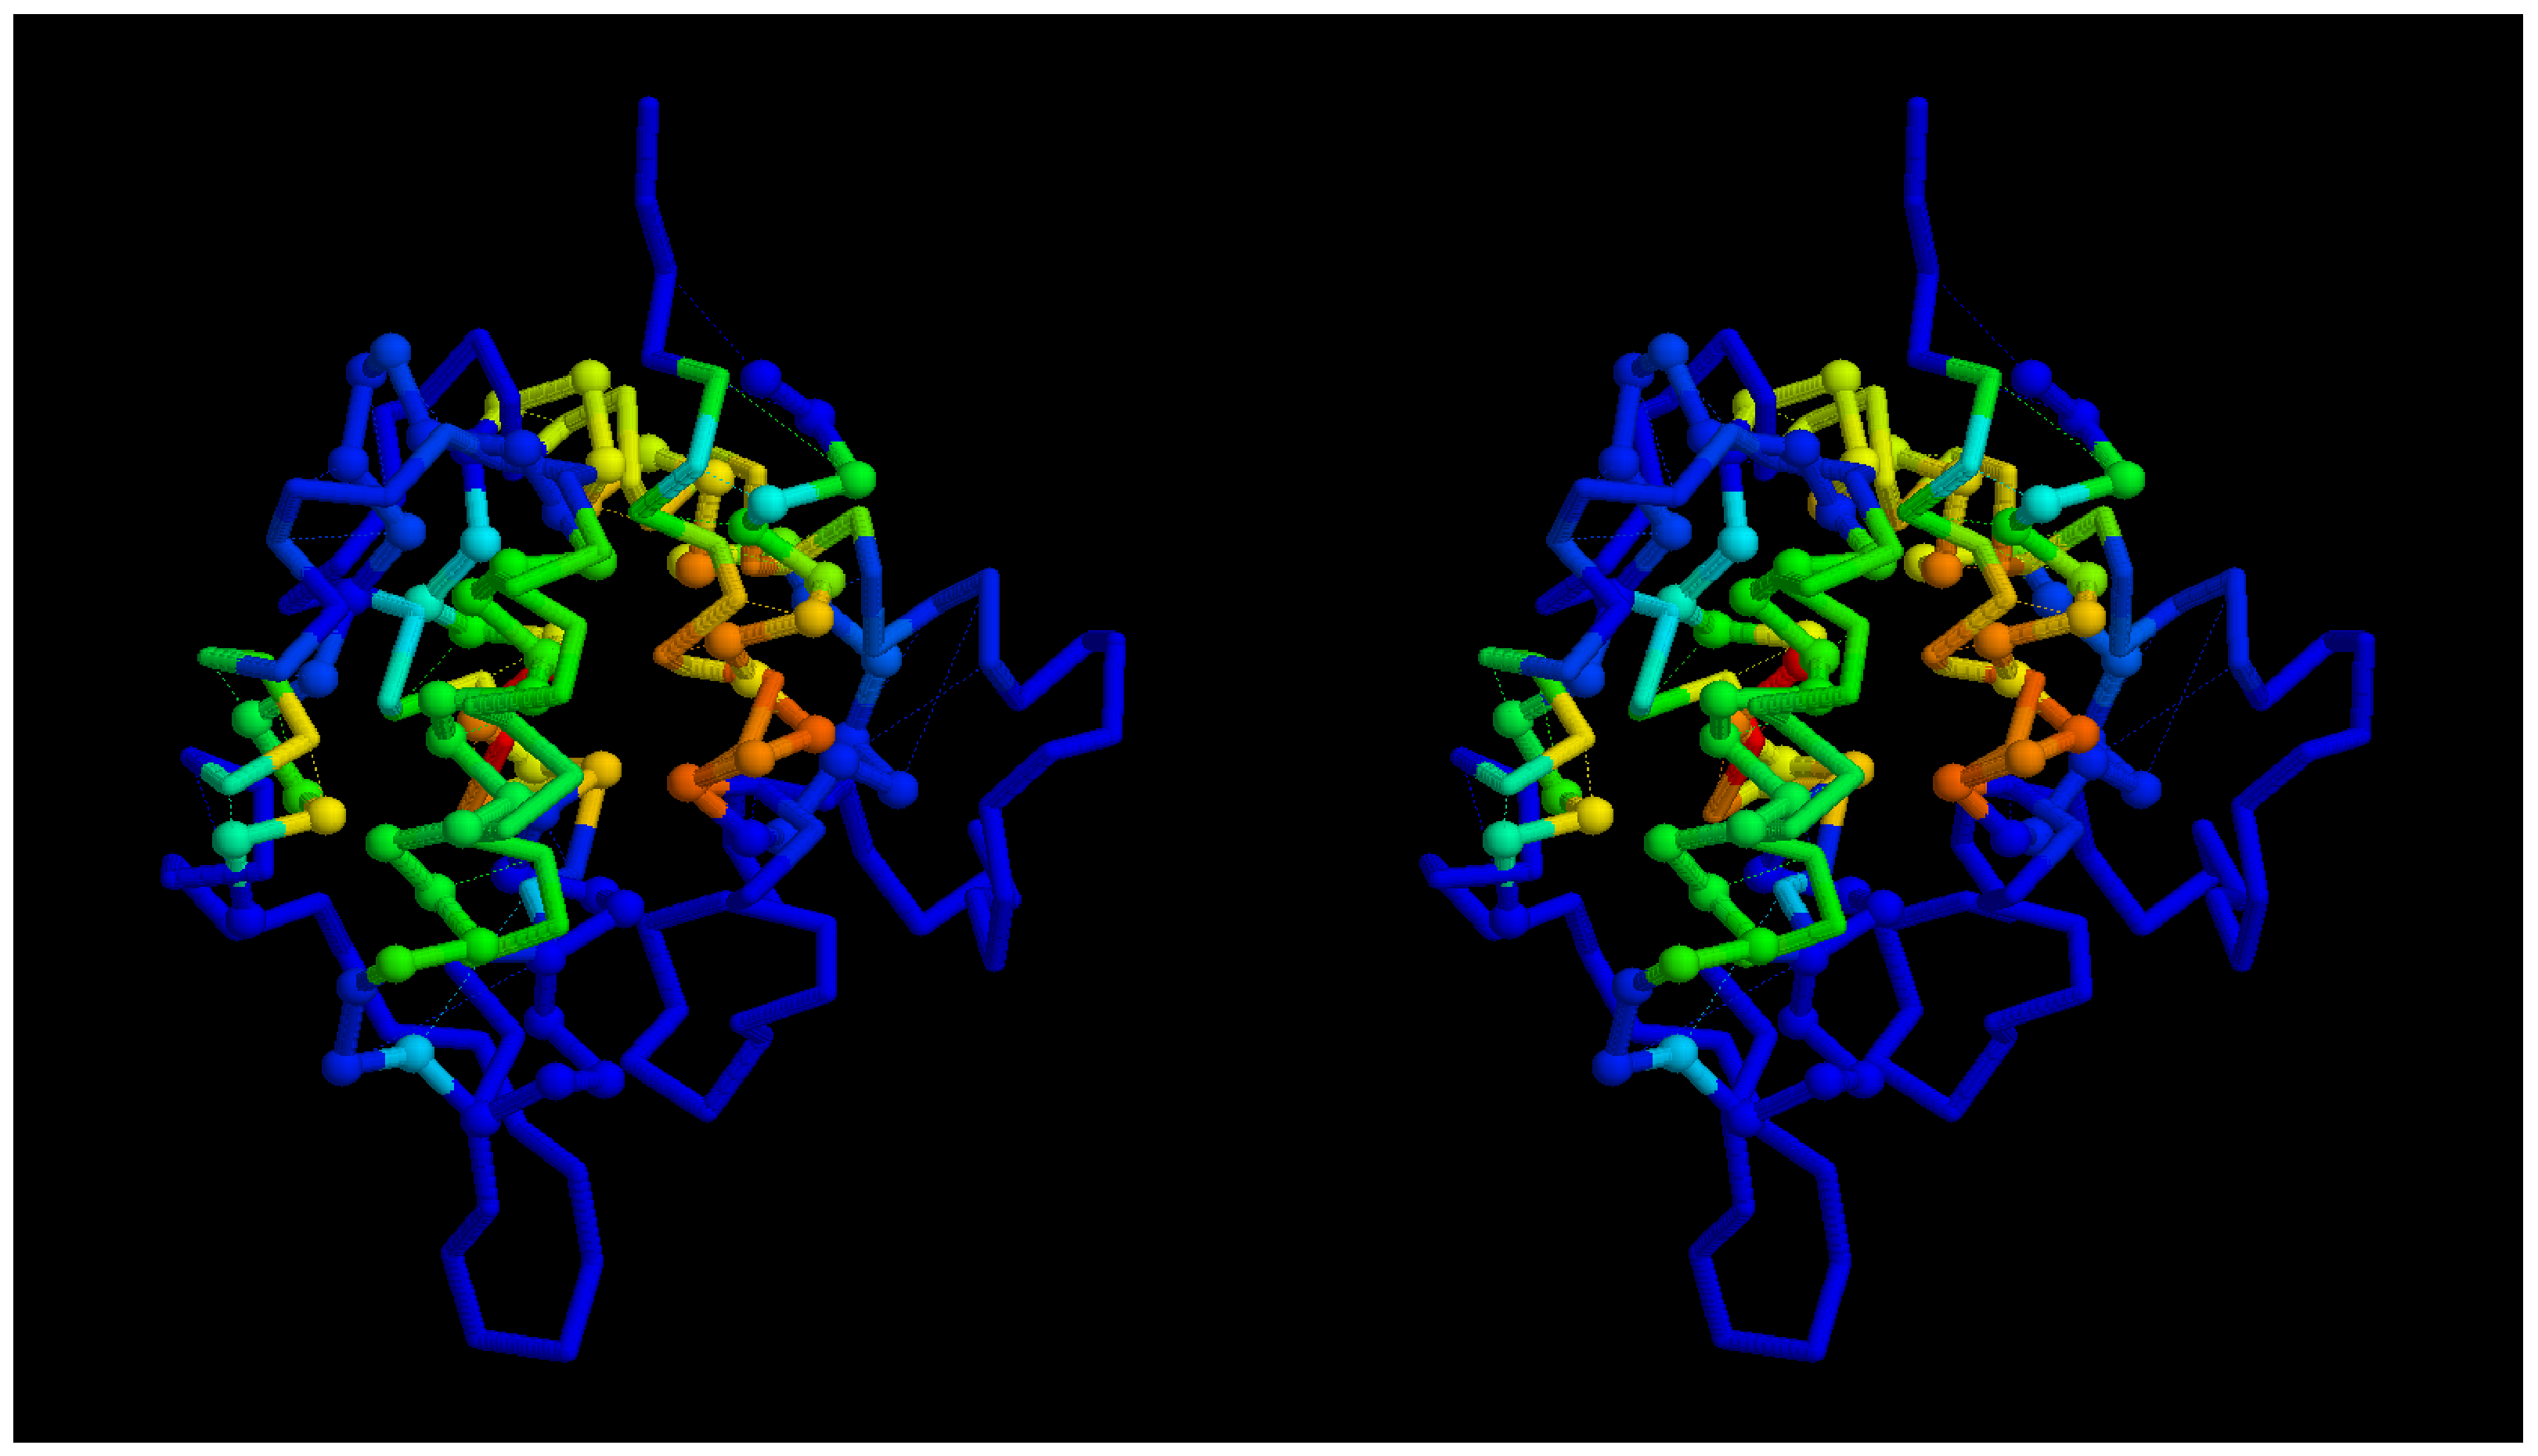
\includegraphics[width=300pt]{orthoNCall-ortho.eps}
}
\subfigure[foamy]{
\includegraphics[width=300pt]{orthoNCall-foamy.eps}
}
\begin{footnotesize}
\caption{
\label{Fig:final}
{\bf Amino and carboxy domains superposed}.
$a$ ortho virus domains and
$b$ foamy virus domains are shown as a stereo pair with
their \CA\ backbones coloured by
the residue similarity score calculated by \SAP. (red = strong similarity, blue = none).
The amino terminal domain is distinguished by small balls on its \CA\ positions and
the amino terminus lies to the top in both panels.
}
\end{footnotesize}
\end{figure}

\subsection{Fold-space representation}

To summarise the structural relationships among the ortho and foamy domains, the matrix
of pairwise comparisons was projected into a three-dimensional fold-space.  (See methods
for details).   This produces a best visual representation of the RMSD values between domains.

As can be seen from \Fig{space}, the N and C domains of the ortho viruses form distinct
clusters with the foamy C domain lying closer to the ortho C-domain cluster.   The foamy
N-domain, however, maintains a fairly equal distance from both ortho domain clusters but
lies closer to its C-terminal partner.

\begin{figure}
\centering
\includegraphics[width=300pt]{foldspace-space.eps}
\begin{footnotesize}
\caption{
\label{Fig:space}
{\bf Fold-space representation of all domains}.
All the viral domains considered in the paper were projected into a 3D fold-space representing
the relationship of their \SAP\ weighted RMSD values.   The domains are coloured as:
foamyN = cyan, foamyC = red, orthoN = green and ortho C = magenta. 
}
\end{footnotesize}
\end{figure}
\clearpage
%\section{Conclusions}

\subsection{Structure comparison}

\subsubsection{Pairwise significance}

The comparison of small domains that are largely composed of \AHs\ presents a challenging problem in how
to interpret the significance of the RMSD values.  As the individual helical secondary structure elements
(SSEs) constitute a sizeable fraction of the domain, it takes only the chance alignment of a few helices
to result in a low RMSD over a large proportion of the structure, giving an apparently meaingful result.  

The use of
the customised decoy sets attempts to avoided this problem by recreating a large number of possible folds
that were generated using the same (reconnected) SSEs.   Moreover, to avoid any chance recreation of native fragments,
each comparison always involved the comparison of a native (forward) chain direction with a reversed chain.
Using these models, a background distribution of decoy/decoy comparisons allowed us to calculate Z-scores
for each native/native comparison with the advantage that every comparison in the background distribution
involved two models with the same length, density and secondary composition as the native pair.
These values indicated a clearly significant relationship between the foamy and ortho structures.   

\subsubsection{Direct or transposed domain order?}

However, the Z-scores did not point to a clear resolution of whether the domains should have a direct
correspondance (NN and CC match) or a transposed relationship (NC and CN) with significant individual
matches found across all pairings.  Testing for a bias towards more significant like-domain pairings (NN,CC)
in the list of similarities ranked by Z-score confirmed the visual bias towards a direct correspondance
but only at a marginal level of significance (around 0.05).  By contrast, the application of a T-test on the
combined raw comparison data returned a very clear distinction between the direct and the transposed
relationships, clearly favouring the more natural forward order.  

Although the `astronomic' probabilities calculated by the T-test seem very convincing, they
must be viewed in the light of the much lower probabilities calculated from the asymmetry
statistics.   Both calculations involve assumptions and are limited by the small number of known
structures so neither can be taken as definitive.    It would seem likely that the ``true'' level of 
significance may lie somewhere between the two results but as both point in the direction of the NN and CC 
domain order, there is no reason to adopt the more unexpected transposed domain order. 

\subsection{Evolutionary implications}

On the basis of these structural comparisons, and a variety of functional assays described elsewhere, we can
conclude that the central domain of the spumavirus Gag gene encodes a polypeptide sequence related to that of
the corresponding region of orthoretroviruses, CA. It therefore seems reasonable to suppose that the last
common ancestor of orthoretroviruses and spumaviruses possessed such a sequence. Moreover this region appears
to be made up from two related subdomains suggesting a gene duplication event in a common precursor.

In our initial search of the foamy virus capsid using the DALI program, we made
the curious observation that the strongest similarity of the foamy virus capsid
was with the ARC protein (Activity-Regulated Cytoskeleton-associated protein) that
is active in neural synaptic growth and activity (and several other developmental associated functions).
The ARC protein has widespread and clear (non-gag) sequence homologues as far back as insects and probably
deeper, giving it a very ancient origin somewhere close to the metazoan root \cite{CampillosMet06}.
If ARC is considered to be a relic of an ancient Ty3/Gypsy retrotransposon \cite{ZhangWet15}, preserved
as a 'living fossil' in the genomes of metazoa, this relationship would suggest an equally
ancient origin for the foamy virus. 

Alternatively,
the foamy viruses may have co-opted an ARC protein to facilitate budding and their escape from the cell.
As it is believed that the Ty3/Gypsy family of intracellular retrotransposons gave rise to retroviruses
\cite{LlorensCet08}, 
it will therefore be of considerable interest to determine whether such elements possess CA proteins with
a two-domain structure. Finally, it is worth noting that the Gag protein of Ty3 is significantly shorter 
that that of the retroviruses and it is possible that the N-terminal domains of the orthoretroviruses 
and spumaviruses were co-opted at different times to facilitate budding from the cell surface. 
If so, the very different structures of this region in the orthoretroviruses and spumaviruses might suggest 
independent acquisition events. 

\section{Conclusions}

\subsection{Structure comparison}

\subsubsection{Pairwise significance}

The comparison of small domains that are largely composed of \AHs\ presents a challenging problem in how
to interpret the significance of the RMSD values.  As the individual helical secondary structure elements
(SSEs) constitute a sizeable fraction of the domain, it takes only the chance alignment of a few helices
to result in a low RMSD over a large proportion of the structure, giving an apparently meaingful result.  

The use of
the customised decoy sets attempts to avoided this problem by recreating a large number of possible folds
that were generated using the same (reconnected) SSEs.   Moreover, to avoid any chance recreation of native fragments,
each comparison always involved the comparison of a native (forward) chain direction with a reversed chain.
Using these models, a background distribution of decoy/decoy comparisons allowed us to calculate Z-scores
for each native/native comparison with the advantage that every comparison in the background distribution
involved two models with the same length, density and secondary composition as the native pair.
These values indicated a clearly significant relationship between the foamy and ortho structures.   

\subsubsection{Direct or transposed domain order?}

However, the Z-scores did not point to a clear resolution of whether the domains should have a direct
correspondance (NN and CC match) or a transposed relationship (NC and CN) with significant individual
matches found across all pairings.  Testing for a bias towards more significant like-domain pairings (NN,CC)
in the list of similarities ranked by Z-score confirmed the visual bias towards a direct correspondance
but only at a marginal level of significance (around 0.05).  By contrast, the application of a T-test on the
combined raw comparison data returned a very clear distinction between the direct and the transposed
relationships, clearly favouring the more natural forward order.  

Although the `astronomic' probabilities calculated by the T-test seem very convincing, they
must be viewed in the light of the much lower probabilities calculated from the asymmetry
statistics.   Both calculations involve assumptions and are limited by the small number of known
structures so neither can be taken as definitive.    It would seem likely that the ``true'' level of 
significance may lie somewhere between the two results but as both point in the direction of the NN and CC 
domain order, there is no reason to adopt the more unexpected transposed domain order. 

\subsection{Evolutionary implications}

On the basis of these structural comparisons, and a variety of functional assays described elsewhere, we can
conclude that the central domain of the spumavirus Gag gene encodes a polypeptide sequence related to that of
the corresponding region of orthoretroviruses, CA. It therefore seems reasonable to suppose that the last
common ancestor of orthoretroviruses and spumaviruses possessed such a sequence. Moreover this region appears
to be made up from two related subdomains suggesting a gene duplication event in a common precursor.

In our initial search of the foamy virus capsid using the DALI program, we made
the curious observation that the strongest similarity of the foamy virus capsid
was with the ARC protein (Activity-Regulated Cytoskeleton-associated protein) that
is active in neural synaptic growth and activity (and several other developmental associated functions).
The ARC protein has widespread and clear (non-gag) sequence homologues as far back as insects and probably
deeper, giving it a very ancient origin somewhere close to the metazoan root \cite{CampillosMet06}.
If ARC is considered to be a relic of an ancient Ty3/Gypsy retrotransposon \cite{ZhangWet15}, preserved
as a 'living fossil' in the genomes of metazoa, this relationship would suggest an equally
ancient origin for the foamy virus. 

Alternatively,
the foamy viruses may have co-opted an ARC protein to facilitate budding and their escape from the cell.
As it is believed that the Ty3/Gypsy family of intracellular retrotransposons gave rise to retroviruses
\cite{LlorensCet08}, 
it will therefore be of considerable interest to determine whether such elements possess CA proteins with
a two-domain structure. Finally, it is worth noting that the Gag protein of Ty3 is significantly shorter 
that that of the retroviruses and it is possible that the N-terminal domains of the orthoretroviruses 
and spumaviruses were co-opted at different times to facilitate budding from the cell surface. 
If so, the very different structures of this region in the orthoretroviruses and spumaviruses might suggest 
independent acquisition events. 
\clearpage
%\section{Methods}

\subsection{Structural data}

The foamy virus structures were obtained from the Protein Structure Databank
(PDB code:{\tt 1ian-A}) \cite{ian}.

The ortho virus structures used, with their shorthand code and PDB code, were:
bovine leukemia virus (BLV) {\tt} \cite{},
bovine leukemia virus (BLV6) {\tt} \cite{},
human immunodeficiency virus 1 (HIV1) {\tt} \cite{},
human endogenous retrovirus type-K (HML2) {\tt} \cite{},
human T-cell leukemia virus (HTLV) {\tt} \cite{},
jaagsiekte sheep Retrovirus (JSRV) {\tt} \cite{},
murine leukemia virus (MLV) {\tt} \cite{},
Mason-Pfizer monkey virus (MPMV) {\tt} \cite{},
{\em Plautia stali} intestine virus (PSIV) {\tt} \cite{},
rabbit endogenous lentivirus type-K (RELIK) {\tt} \cite{},
Rous sarcoma virsu (RSV) {\tt} \cite{}.

\subsection{Structure comparison}

\subsubsection{\DALI}

The \DALI\ method for searching the PDB with a structural query \cite{HolmLet93,HolmLet}
was accesed via the server at:
{\tt http://ekhidna.biocenter.helsinki.fi/dali\_server}.
The \DALI\ method reports the significance of each match with an estimated Z-score
which is the raw comparison score, normalised by the combined length of the proteins.
Z-scores down to a value of 2 are reported by the program.

The list of \DALI\ hits (ranked by Z-score) were assessed by how many high-scoring capsid structures had
been identified.    These true/false (T/F) hits were defined simply by protein descriptions that contained the
words "CAPSID", "GAG" or "P24".   This may have misclassified a few (low scoring) hits to the matrix protein
and missed some hits where the primary description refers to a cyclophilin structure solved in complex 
with the capsid. 

\DALI\ reports structural hits in both the full PDB and a reduced collection of structures that
have no pair of proteins with over 90\% sequence identity, ireferred to as the 90\%non-redundant or PDB-90 collection.
It was found, however, that some hits, seen in the full PDB were not found in the PDB-90, for example in \Fig{revs},
all of the top 31 hits of the N-domain against the full PDB are missing in the PDB-90 hits.
The most likely explanation is that the PDB-90 secection has not been updated at the same time
as the full collection.    For this reason, hits to both databases were monitored.

\subsubsection{\SAP}

The \SAP\ method for structure comparison \cite{TaylorWR99a} was run as local copy which can
be accessed at: {\tt mathbio}.   As part of determining the alignment between two structures,
the \SAP\ program calculates a similarity score for each pair of matched positions which is
how similar the rest of the structure looks from the viewing-frame of the superposed residues.
This value can be used both to weight the importance of positions when calculating the
(rigid-body) RMSD superposition and to colour positions the superposed structures.
\cite{}. (As in \Fig{}).

If the matched positions are ranked by this value, then RMSD values can be calculated over
increasingly larger subsets to high-light, say, the extent of a well matched core before
the contribution of variable loops, or domain shifts, leads to higher RMSD values.
(As in \Fig{fullRMS}).

\subsection{Decoy structure construction}

\subsubsection{Reversed structure decoys}

Simple structural decoys were generated from native PDB structures by reversing the order
of the \CA\ atoms in the PDB file using the Unix command line:
\begin{verbatim}
cat native.pdb | grep ' CA ' | sort -nr -k2 > reverse.pdb
\end{verbatim}
The reversal of a protein chain does not alter the chirality of the alpha helix and
these decoys can be used directly in \SAP.   However, \DALI\ requires all main-chain atoms
and these must be regenerated for the reversed decoys.   This was done using the simple
{\tt ca2main} program which can also be found at: {\tt  mathbio}.

\subsubsection{Customised decoys}

Customised structural decoys were generated for each comparison using each of the
pair of structures being compared to create two pools of decoys then comparing all
decoys in the first pool against all decoys from the second but with their chain
reversed as described in the previous section.

The decoys were created as described by Taylor \cite{}, starting by cyclising the
chain then introducing new termini in each surface loop to create cyclic permutations.
In addition, when two loop regions lie in close proximity, their ends are also 
swapped.   That is: if a chain runs from amino (N) to carboxy (C) termini through
three adjacent loop regions {\tt a-b} {\tt c-d} and {\tt e-f} as: N,{\tt a-b,c-d,e-f},C
then the swapped chain runs: N,{\tt a-d,e-b,c-f},C with the switch being made at the
least disruptive point.   This swap does not create any reversed segments which would
otherwise form regions of local matching when the whole chain is reversed.

In a pair of structures, if each have four surface loops where breaks can be made, then
including the native termini, this gives five cyclic permutations and if two pairs of 
loops can be reconnected then a total of 15 distinct decoys can be made from each native
starting structure.   As these can be compared pairwise, a pool of 225 decoy derived
data points is generated that constitutes the random background against which the native/native
comparison can be assessed.

For example, in \Fig{sapit}, the 36 data
points marked by a solid circle come from the comparison of six cyclic permutations of a 
native ortho domain compared with six permutations of a reversed foamy domain that includes
a single loop reconnection.  

Every pair drawn from this pool will have the same lengths as the two native structures
as well as the same secondary structure composition, surface exposure and inertial properties
but each decoy will have a different chain fold.


\subsection{Statistical tests}

\subsubsection{RMSD length normalisation}

The quality of structure comparisons can be characterised by a combination of their
RMSD value and the number of matched (superposed) positions.  How to combine these values has
been the subject of much discussion over the years and central to this is the expected random
RMSD value for two proteins of a given length \cite{Mclaughlin,Cohen,Crippen}.   However,
when reviewed \cite{Taylor}, all these measures were approximations of a simple square-root function of
the protein length (as originally proposed by McLachlin on theoretical grounds \cite{McLachlin})
but with an added term to depress the RMSD values obtained with small units or structure
that are dominated by secondary structure elements (and super-secondary structure motifs) 
giving a lower than expected RMSD value.   The formula that best captures this is:
$R = \surd N (1-\exp(-N^2/s^2))$,
where,
$R$ is the expected random RMSD for $N$ matched positions and $s$ is the damping factor in the inverted
Gaussian term (equivalent to the standard deviation in the Normal distribution).  

Any point that lies on this line can be considered "exactly" random
with those above it being "more" random and those below it "less" random.  This can be quantified
as a single number which is the value of a scaling factor ($a$), which when applied to the curve, makes it
pass through any given point.   If a comparison has an RMSD of $R$ over $N$ positions, then
$R = a\surd N (1-\exp(-N^2/s^2))$ and when
\begin{equation}
\label{Eqn:fit}
a = R/(\surd N (1-\exp(-N^2/s^2))), 
\end{equation}
the line will pass through the data point.  This reduces the pair of values ($R,N$) to a
single value $a$ that is a simpler quantity for statistical analysis.

The best value for $s$ is slightly dependent on the nature of the proteins being compared.
For artifical (random-walk)  models with no secondary structure, no modification will be needed but the
proteins considered here have segments of packed alpha helices that can be locally similar
over two to three helices.   To correct for this, a value of $s=30$ was used (or $1/s^2 = 0.11$)
which is higher than the value of $1/s^2 = 0.03$ used previously.
That this is a reasonable fit to the data can be seen in the way the dashed blue lines
in \Fig{sapit} track the upper and lower boundary of the decoy comparison results.

When $a=1$, the point lies on the random line and when $a=0$, the RMSD is zero, so values of
$a$ that approach this lower bound will be of interest when evaluating similarity. 

\subsubsection{Frequency plots}

The $a$-values obtained using \Eqn{fit} were plotted as frequency histograms using using
only data points that had a length of $N\pm 10$, where $N$ is the maximum number of matched
positions.   Previously, a cumulative plot of RMSD was used to select an optimal value for
$N$ (giving the minimum $a$-value).   This can be important if the full set of matched
positions is dominated by a high deviations from variable loop regions.   However, in the
current application, the small length of the foamy virus loops meant that this was not
an important aspect and the full number of matched positions was taken.   Otherwise, the
same correction would have to be applied to all decoy comparisons to maintain a fair
comparison.  (See \Fig{sapit}, where the black dot marks the minimum $a$-value length).

The mean and standard deviation of the $a$-values in the $N\pm10$ region were calculated
and the corresponding Normal distribution used to calculate Z-scores for the associated
native comparison. (See \Fig{normHIV}, for an example).

\subsubsection{T-tests}

Data from separate native/native comparisons, with their customised decoy data, were combined
giving not only a much larger background decoy derived population of scores but also a smaller
distribution of native comparison scores that can be tested to calculate the probability that
they were drawn from the same population as the decoy data.  To do this, a T-test was used which
takes the size, mean, and standard deviation of each distribution and calculates a probability.
The implementaion of this test was taken from the the Numerical Reicpies collection \cite{}
which implements one of two variants of the test depending on whether the distributions
have statistically distinct standard deviations. (Routines {\tt ttest()} and {\tt tutest()}).  
The choice of routine is based on a preapplication of an F-test on the standard-deviations. 
(Using the routine {\tt ftest()}).

The values quoted in the Results section are for a two-tailed T-test, however, as it is expected
that the native comparisons should always be more similar than comparisons between random models,
then a one-tailed T-test would be valid, which gives half the probability.   As the values
in the Tables are so significant and only the relative relationships are of interest,
then the choice is unimportant.

\subsection{Fold-space clustering}

The results of the pairwise similarity within a set of structures can be visualised by treating the
RMSD values as Euclidean distances\footnote{In theory, pairwise RMSD values are guaranteed to constitute 
a consistent Euclidean metric, but only in N-1 dimensions (where N is the number of structures compared).
} and reducing their dimensionaliy to sufficiently few dimensions to be visualised: usually 2 or, better 3,
to visualise the space with less distortion.
Rather than use a simple multi-dimensional scaling (MDS) method (\cite{BrownNPet96}), the more complicated 
method of multi-dimensional projection was used (\cite{AszodiAet97a}, see \cite{TaylorWRet01b} for a
simpler exposition).  

This method reduces the dimensionality of the projection in gradual stages
with each step employing triangle-inequality balancing and hyper-dimensional real-space refinement.
In the real-space refinement stages, a weight can be applied to pairwise distances. (This cannot be
done in direct MDS projection, which can only assign a mass to each point).  
Weights were assigned to distances as a function of their inverse RMSD, up to a maximum value of 1.

The method is robust and
has been widely applied to rough models (\cite{TaylorWRet09a}) and predicted inter-residue distances that 
constitute highly non-metric data sets (\cite{AszodiAet94a}).


\section{Methods}

\subsection{Structural data}

The foamy virus structures were obtained from the Protein Structure Databank
(PDB code:{\tt 5M1G}) \cite{BallNJet16}.

%wtaylor@wt:~/ianpdbs/notes$ cat pdbid.ian
%
%N-terminal orthoretroviral CA domains
%1) Ortho-HIV1_NtD.pdb – (Lentivirus) Taken from HIV-Cyp structure. PDB code 1AK4.
%2) Ortho_HML2_NtD.pdb – (Betaretrovirus) crystal structure of NtD of human endogenous virus HML2, our unpublished structure.
%3) Ortho_HTLV_NtD.pdb – (Deltaretrovirus) NMR structure of HTLV CA-NtD. Resolution a bit poor and N-terminal beta hairpin not correctly modelled. PDB code 1G03.
%4) Ortho_JSRV_NtD.pdb – (Betaretrovirus) Our X-ray structure of CA-NtD from JSRV. PDB code 2V4X
%5) Ortho_MLV_NtD – (gammaretrovirus) one monomer taken from our X-ray structure of N-MLV. PDB code 1U7K
%6) Ortho_MPMV_NtD – (betaretrovirus) NMR structure of CA NtD domain from MPMV. PDB code 2KGF
%7) Ortho_RSV_NtD.pdb – (alpharetrovirus) One Ntd Monomer taken from RSV CA –NtD crystal dimer. PDB code 1EM9
%8) Ortho_BLV_NtD.pdb – (Deltaretrovirus) One NtD monomer taken from a BLV NtD crystal dimer. PDB code 4PH2
%9) Ortho_RELIC_NtD.pdb – (Lentivirus, ancient) One Ntd monomer Taken from our X-ray structure of a RELIK crystal dimer. PDB code 2XGU.
%10) ortho_PSIV_NtD.pdb – (Lentivirus, ancient) Ntd monomer in our X-ray crystal structure of PSIV. PDB code 2XGU.
%
%C-terminal orthoretroviral CA domains
%1) Ortho_HIV1_CtD – (Lentivirus) One CtD monomer taken from an HIV1 crystal dimer crystal. PDB code 1A43
%2) Ortho_RSV_CtD.pdb – (Alpharetrovirus) One Ctd Monomer taken from RSV CtD crystal dimer. PDB code 3G1I. This dimer was neural pH. There are other forms at high and low pH.
%3) BLV_CA_CtD.pdb – (Deltaretrovirus) One CtD monomer taken from a BLV CtD crystal trimer. PDB code 4PH1.
%4) Ortho_HML2_CtD.pdb – (Betaretrovirus) Our NMR structure of CtD of human endogenous virus HML2, our unpublished structure.
%Orthoretroviral CA domains
%1) Ortho_HIV1_CA_hex_P6.pdb – (Lentivirus) One CA monomer out of a P6 disk. PDB code 3H47.
%2) Ortho_HIV1_CA_hex_P212121 – (Lentivirus) One CA monomer extracted out of a hexameric disk. PDB code 3H4E.
%3) Ortho_HTLV_CA.pdb _ (Deltaretrovirus) NMR structure of HTLV CA. PDB code 1QRJ.
%4) Ortho_BLV_CA_Hex_P65.pdb. – (Deltaretrovirus) One CA monomer extracted out of a hexameric disk. PDB code 4PH0.

The ortho virus structures used, with their shorthand code in bold and PDB code in teletype, were:
\begin{itemize}
\item {\bf BLV}:  bovine leukemia virus (deltaretrovirus) {\tt 4PH1} (N-ter.dom) and {\tt 4PH2} (C-ter.dom) \cite{ObalGet15},
\item {\bf BLV6}: bovine leukemia virus (hexameric) {\tt 4PH0} (both dom.s) \cite{ObalGet15},
\item {\bf HIV1}: human immunodeficiency virus 1 (lentivirus) {\tt 1AK4} (N-ter.dom) \cite{GambleTRet96} and {\tt 1A43} (C-ter.dom) \cite{WorthylakeDKet99},
\item {\bf HIV6}: human immunodeficiency virus 1 {\tt 3H47} (both dom.s) \cite{PornillosOet09},
\item {\bf HML2}: human endogenous retrovirus type-K (betaretrovirus) {\tt } \cite{MortuzaGBet08},
\item {\bf HTLV}: human T-cell leukemia virus (deltaretrovirus) {\tt 1QRJ} (both dom.s) \cite{KhorasanizadehSet99},
\item {\bf JSRV}: jaagsiekte sheep Retrovirus (betaretrovirus) {\tt 2V4X} (N-ter.dom) \cite{MortuzaGBet09},
\item {\bf MLV}:  murine leukemia virus (gammaretrovirus) {\tt 1U7K} (N-ter.dom) \cite{MortuzaGBet04},
\item {\bf MPMV}: Mason-Pfizer monkey virus (betaretrovirus) {\tt 2KGF} (N-ter.dom) \cite{MacekPet09},
\item {\bf PSIV}: prosimian immunodefficiency virus (ancient lentivirus) {\tt 2XGV} (N-ter.dom) \cite{GoldstoneDCet10},
\item {\bf RELIK}: rabbit endogenous lentivirus type-K (ancient lentivirus) {\tt 2XGU} (N-ter.dom) \cite{GoldstoneDCet10},
\item {\bf RSV}:  Rous sarcoma virus (alpharetrovirus) {\tt 3G1I} (both dom.s) \cite{BaileyGDet09}.
\end{itemize}

\subsection{Structure comparison}

\subsubsection{\DALI}

The \DALI\ method for searching the PDB with a structural query \cite{HolmLet93a}
was accesed via the server at:
{\tt http://ekhidna.biocenter.helsinki.fi/dali\_server}.
The \DALI\ method reports the significance of each match with an estimated Z-score
which is the raw comparison score, normalised by the combined length of the proteins.
Z-scores down to a value of 2 are reported by the program.

The list of \DALI\ hits (ranked by Z-score) were assessed by how many high-scoring capsid structures had
been identified.    These true/false (T/F) hits were defined simply by protein descriptions that contained the
words "CAPSID", "GAG" or "P24".   This may have misclassified a few (low scoring) hits to the matrix protein
and missed some hits where the primary description refers to a cyclophilin structure solved in complex 
with the capsid. 

\DALI\ reports structural hits in both the full PDB and a reduced collection of structures that
have no pair of proteins with over 90\% sequence identity, referred to as the 90\% non-redundant or PDB-90 collection.
It was found, however, that some hits, seen in the full PDB were not found in the PDB-90, for example in \Fig{revs},
all of the top 31 hits of the N-domain against the full PDB are missing in the PDB-90 hits.
The most likely explanation is that the PDB-90 secection has not been updated at the same time
as the full collection.    For this reason, hits to both databases were monitored.

\subsubsection{\SAP}

The \SAP\ method for structure comparison \cite{TaylorWR99a} was run as local copy which can
be accessed at: {\tt mathbio}.   As part of determining the alignment between two structures,
the \SAP\ program calculates a similarity score for each pair of matched positions which is
how similar the rest of the structure looks from the viewing-frame of the superposed residues.
This value can be used both to weight the importance of positions when calculating the
(rigid-body) RMSD superposition and to colour positions in the superposed structures.
\cite{RippmannFet91a}. (As in \Fig{top2}).

If the matched positions are ranked by this value, then RMSD values can be calculated over
increasingly larger subsets to high-light the extent of a well matched core before
the contribution of variable loops, or domain shifts, leads to higher RMSD values.
(As in \Fig{fullRMS}).

\subsection{Decoy structure construction}

\subsubsection{Reversed structure decoys}

Simple structural decoys were generated from native PDB structures by reversing the order
of the \CA\ atoms in the PDB file using the Unix command line:
\begin{verbatim}
cat native.pdb | grep ' CA ' | sort -nr -k2 > reverse.pdb
\end{verbatim}
The reversal of a protein chain does not alter the chirality of the alpha helix and
these decoys can be used directly in \SAP.   However, \DALI\ requires all main-chain atoms
and these must be regenerated for the reversed decoys.   This was done using the simple
{\tt ca2main} program which can also be found at: {\tt  mathbio}.

\subsubsection{Customised decoys}

Customised structural decoys were generated for each comparison using each of the
pair of structures being compared to create two pools of decoys then comparing all
decoys in the first pool against all decoys from the second but with their chain
reversed as described in the previous section.

The decoys were created as described by Taylor \cite{TaylorWR06a}, starting by cyclising the
chain then introducing new termini in each surface loop to create cyclic permutations.
In addition, when three loop regions lie in close proximity, their ends are also 
swapped.   That is: if a chain runs from amino (N) to carboxy (C) termini through
three adjacent loop regions {\tt a-b}, {\tt c-d} and {\tt e-f} as: N,{\tt a-b,c-d,e-f},C
then the swapped chain runs: N,{\tt a-d,e-b,c-f},C with each switch being made at the
least disruptive point.   This swap does not create any reversed segments which would
otherwise form regions of local matching when the whole chain is reversed.

In a pair of structures, if each have four surface loops where breaks can be made, then
including the native termini, this gives five cyclic permutations and if two groups of 
loops can be reconnected then a total of 15 distinct decoys can be made from each native
starting structure.   As these can be compared pairwise, a pool of 225 decoy derived
data points is generated that constitutes the random background against which the native/native
comparison can be assessed.

For example, in \Fig{sapit}, the 36 data
points marked by a solid circle come from the comparison of six cyclic permutations of a 
native ortho domain compared with six permutations of a reversed foamy domain that includes
a single loop reconnection.  

Every pair drawn from this pool will have the same lengths as the two native structures
as well as the same secondary structure composition, surface exposure and inertial properties
but each decoy will have a different chain fold.


\subsection{Statistical tests}

\subsubsection{RMSD length normalisation}

The quality of structure comparisons can be characterised by a combination of their
RMSD value and the number of matched (superposed) positions.  How to combine these values has
been the subject of much discussion over the years and central to this is the expected random
RMSD value for two proteins of a given length \cite{McLachlanAD84,CohenFEet80d,MaiorovVNet94}.   However,
when reviewed \cite{TaylorWR06a}, all these measures were approximations of a simple square-root function of
the protein length (as originally proposed by McLachlan on theoretical grounds \cite{McLachlanAD84})
but with an added term to depress the RMSD values obtained with small units or structure
that are dominated by secondary structure elements (and super-secondary structure motifs) 
giving a lower than expected RMSD value.   The formula that best captures this is:
$R = \surd N (1-\exp(-N^2/s^2))$,
where,
$R$ is the expected random RMSD for $N$ matched positions and $s$ is the damping factor in the inverted
Gaussian term (equivalent to the standard deviation in the Normal distribution).  

Any point that lies on this line can be considered "exactly" random
with those above it being "more" random and those below it "less" random.  This can be quantified
as a single number which is the value of a scaling factor ($a$), which when applied to the curve, makes it
pass through any given point.   If a comparison has an RMSD of $R$ over $N$ positions, then
$R = a\surd N (1-\exp(-N^2/s^2))$ and when
\begin{equation}
\label{Eqn:fit}
a = R/(\surd N (1-\exp(-N^2/s^2))), 
\end{equation}
the line will pass through the data point.  This reduces the pair of values ($R,N$) to a
single value $a$ that is a simpler quantity for statistical analysis.

The best value for $s$ is slightly dependent on the nature of the proteins being compared.
For artifical (random-walk)  models with no secondary structure, no modification will be needed but the
proteins considered here have segments of packed alpha helices that can be locally similar
over two to three helices.   To correct for this, a value of $s=30$ was used (or $1/s^2 = 0.11$)
which is higher than the value of $1/s^2 = 0.03$ used previously.
That this is a reasonable fit to the data can be seen in the way the dashed blue lines
in \Fig{sapit} track the upper and lower boundary of the decoy comparison results.

When $a=1$, the point lies on the random line and when $a=0$, the RMSD is zero, so values of
$a$ that approach this lower bound will be of interest when evaluating similarity. 

\subsubsection{Frequency plots}

The $a$-values obtained using \Eqn{fit} were plotted as frequency histograms using using
only data points that had a length of $N\pm 10$, where $N$ is the maximum number of matched
positions.   Previously, a cumulative plot of RMSD was used to select an optimal value for
$N$ (giving the minimum $a$-value).   This can be important if the full set of matched
positions is dominated by a high deviations from variable loop regions.   However, in the
current application, the small length of the foamy virus loops meant that this was not
an important aspect and the full number of matched positions was taken.   Otherwise, the
same correction would have to be applied to all decoy comparisons to maintain a fair
comparison.  (See \Fig{sapit}, where the black dot marks the minimum $a$-value length).

The mean and standard deviation of the $a$-values in the $N\pm10$ region were calculated
and the corresponding Normal distribution used to calculate Z-scores for the associated
native comparison. (See \Fig{normHIV}, for an example).

\subsubsection{T-tests}

Data from separate native/native comparisons, with their customised decoy data, were combined
giving not only a much larger background decoy derived population of scores but also a smaller
distribution of native comparison scores that can be tested to calculate the probability that
they were drawn from the same population as the decoy data.  To do this, a T-test was used which
takes the size, mean, and standard deviation of each distribution and calculates a probability.
The implementaion of this test was taken from the Numerical Reicpies collection \cite{PressWHet86}
which implements one of two variants of the test depending on whether the distributions
have statistically distinct standard deviations. (Routines {\tt ttest()} and {\tt tutest()}).  
The choice of routine is based on a preapplication of an F-test on the standard-deviations. 
(Using the routine {\tt ftest()}).

The values quoted in the Results section are for a two-tailed T-test, however, as it is expected
that the native comparisons should always be more similar than comparisons between random models,
then a one-tailed T-test would be valid, which gives half the probability.   As the values
in the Tables are so significant and only the relative relationships are of interest,
then the choice is unimportant.

\subsection{Fold-space clustering}

The results of the pairwise similarity within a set of structures can be visualised by treating the
RMSD values as Euclidean distances\footnote{In theory, pairwise RMSD values are guaranteed to constitute 
a consistent Euclidean metric, but only in N-1 dimensions (where N is the number of structures compared).
} and reducing their dimensionality to sufficiently few dimensions to be visualised: usually 2D or, 
better 3D, to visualise the space with less distortion.
Rather than use a simple multi-dimensional scaling (MDS) method (\cite{BrownNPet96}), the more complicated 
method of multi-dimensional projection was used (\cite{AszodiAet97a}, see \cite{TaylorWRet01b} for a
simpler exposition).  

This method reduces the dimensionality of the projection in gradual stages
with each step employing triangle-inequality balancing and hyper-dimensional real-space refinement.
In the real-space refinement stages, a weight can be applied to pairwise distances. (This cannot be
done in direct MDS projection, which can only assign a mass to each point).  
Weights were assigned to distances as a function of their inverse RMSD, up to a maximum value of 1.

The method is robust and
has been widely applied to rough models (\cite{TaylorWRet09a}) and predicted inter-residue distances that 
constitute highly non-metric data sets (\cite{AszodiAet94a}).

\clearpage
\begin{singlespace}
\bibliographystyle{latex/jtb}
\bibliography{latex/newrefs,pdbrefs}
\paragraph{Acknowledgements:}
The work was supported by the Francis Crick Institute under awards: 000000 (WRT), 000000 (JPS) and 000000 (IAT). 
The Crick receives its core funding from Cancer Research UK, the UK Medical Research Council, and the Wellcome Trust.
%\clearpage
%\include{appendix}
\end{singlespace}
\end{document}
